\chapter{System Description}
\label{cha:system-description}

This chapter describes the Kukui Cup system. By system, I mean all aspects of the 2011 UH Kukui Cup: the energy conservation competition, the point competition, the events that took place during the challenge, and the underlying information infrastructure that supported it.

The 2011 Kukui Cup was designed with three goals in mind:

\begin{enumerate}
	\item Enabling research into fostering sustainable environmental behavior change;
	\item Improving the energy literacy of the participants; and
	\item Reducing the energy consumption of the residence halls.
\end{enumerate}

The participants competed in two ways: to reduce energy consumption in the participating residence halls, and to accumulate points by performing tasks related to energy literacy and conservation through the challenge website.

\section{Setting}
\label{sec:setting}

The 2011 Kukui Cup took place in the Hale Aloha residence halls on the University of \Hawaii at \Manoa campus~\cite{hale-aloha-website}. Hale Aloha consists of four cylindrical towers, named after \Hawaiian flowers: Lehua, Ilima, Mokihana, and Lokelani. The towers are arranged around a central courtyard that contains benches, trees, and small raised platform that can be used as a stage. Next to the courtyard is a large cafeteria that provides meals for all the on-campus student residents.

The Hale Aloha towers were built in the 1970s. Each tower contains 13 floors with the following composition:

\begin{itemize}
	\item Floor 1: lobby (front desk, mailboxes, vending machine, TV)
	\item Floor 2: apartment for a Residence Director or Assistant Residence Director
	\item Floors 3--12: rooms for student residents
	\item Floor 13: laundry room, shared kitchen, meeting \& study spaces
\end{itemize}

The student resident floors (3--12) contain 14 inhabited rooms: 13 rooms intended for two residents, and one room designated for the floor's Resident Advisor (RA), who lives alone. There are two bathrooms per floor, each containing multiple individual rooms with a shower, toilet, and sink with a lockable door.

The even floors (4, 6, 8, 10, 12) have a sunken lounge space in the center of the floor with chairs, tables, and benches. The odd floors (3, 5, 7, 9, 11) share the lounge with the even floor above, accessed by a central stairwell. The pairs of floors are called ``lounges'' after their shared lounge space and labeled by letter: lounge A (3--4), lounge B (5--6), lounge C (7--8), lounge D (9--10), and lounge E (11--12). Hereafter, a lounge (pair of floors) will be specified using the name of the tower and the letter of the lounge, such as Ilima A or Lokelani C. With four towers, each containing five lounges, there are a total of 20 lounges participating in the challenge.

There are two elevators in each tower: one that serves each floor (1--12), and one that goes only to the lounges (A--E and R, the roof lounge that is the 13th floor).

The residents' rooms include a pair of beds, armoires, desks, and chairs with one set arranged along each wall. In Lehua and Ilima, each side of the room has two power outlet boxes (4 outlets), while Mokihana and Lokelani have three power outlet boxes (6 outlets). Each room has two Ethernet jacks that provide Internet access. The student resident floors have have no central air conditioning, relying on windows for climate control (due to \Hawaii's climate, there is no need for heating). Residents with special needs (such as breathing problems or severe allergies) may request the installation of a room air conditioner at additional cost beyond the standard housing rates. There were three such air conditioning units approved during the Fall 2011 semester. Unapproved air conditioners are not allowed, and residents caught with one must pay a fine for energy consumption based on the number of weeks it was present in the room.


\section{Participants}
\label{sec:participants}

The participants of the challenge were the residents of the four Hale Aloha towers. The residents were all first-year students starting at UH \Manoa. Each resident floor was overseen by a Resident Advisor (RA), a paid student employee who was in charge of enforcing rules, organizing activities, and being the first point of contact for residents. The RAs were allowed and encouraged to participate in and promote the challenge.

These first-year student residence halls are specifically targeted for two reasons. First, based on conversations with UH \Manoa undergraduates, residents in the first-year residence halls are more likely to attend floor meetings and events, while upper-class residence halls are more like apartments where residents might not know their neighbors well or be motivated to attend floor meetings. Second, as the goal is to improve energy literacy and foster behavior changes in the participants, the earlier these changes take place in their college experience, the more benefit there will be to the participants and the University.

Each floor of the Hale Aloha towers has an RA and 13 double occupancy rooms, and there are 10 floors of student residents per tower. Therefore, at full occupancy, there are 270 potential participants per tower and 1080 potential participants in total.

The challenge was run by a team of Kukui Cup staff, which included a professor, graduate and undergraduate students. The staff organized and ran events, put up marketing posters, and administered the challenge website.


\section{Timing}

The 2011 Kukui Cup was organized into three rounds, each lasting a week. Two to three week student housing energy competitions are common (such as the one described by Petersen et al.~\cite{petersen-dorm-energy-reduction}), and provide a balance between sufficient time to get participants involved and waning interest in a longer challenge. The intensive event schedule, need for fresh energy literacy content, and logistical overhead of running the challenge also made a longer challenge infeasible for this inaugural Kukui Cup.

As discussed in \autoref{sec:participants}, the Kukui Cup took place in first-year residence halls in an attempt to increase participation by students just starting in a new environment, and hopefully thereby more receptive to new experiences. For this same reason, we wanted to hold the challenge in the Fall semester, in the first half of participants' first year. The Fall semester at UH \Manoa starts in late August (August 22 in 2011), and ends in mid-December (December 15 in 2011). We scheduled the challenge in the middle of the semester for two reasons. First, at the beginning of the semester students are settling into their new environment and dealing with their classes. I also needed time to gather baseline data on electricity usage before the challenge started, precluding an early semester start. Second, starting late in the semester is complicated by the Thanksgiving holiday (which took place during the week of November 22 in 2011), and the increasing workload as the semester winds down. The 2011 challenge started at midnight on Sunday October 16, 2011 and ended at midnight on Sunday November 7, 2011.


\section{Energy Meters}
\label{sec:energy-meters}

Monitoring the energy use by the residents is a core aspect of this research. This section covers the physical infrastructure needed to monitor energy use. Note that in the Hale Aloha towers, electricity is the only real source of energy in use (there is no natural gas or heating oil use). Therefore the energy monitoring is limited to monitoring of electricity use, and the terms energy and electricity are used interchangeably throughout this document.


\subsection{Meter Operation Principles}

Power meters typically work by sampling the voltage and current passing through a circuit to compute the power being consumed or produced ($Power = Current \times Voltage$). In a building setting, a meter will often measure the power being used by a single electrical distribution panel, which contains circuit breakers for the various loads in the vicinity. While voltages may be measured directly by connecting a voltmeter to one of the breakers, often the current present in home or institutional wiring are too large for convenient measurement by a meter. Current transformers (CTs) are used to step down this higher current to a more useable level. CTs are torus-shaped and typically have two pieces that can be clamped around existing wiring, allowing installation without breaking the existing electrical circuit. In an institutional setting, typically three-phase power will be used since it is a more economical use of conductor for heavy loads compared to single or two-phase power. To measure three-phase power, typically three ammeters (and thereby three CTs) and one voltmeter are required. A digital power meter will sample these four inputs at high frequency to compute power use, and also integrate over time to compute energy use (see \autoref{app:power-energy} for an explanation of the difference between power and energy).\fxnote{Add photo of meter and CTs}


\subsection{Meter Selection}
\label{sec:meter-selection}

The Kukui Cup energy competition required two uncommon features for the energy metering: monitoring at the level of a floor as opposed to a whole building, and near real-time data collection at approximately 15 second intervals. In addition, we required that the meter provide a documented way to retrieve the energy data so that I could write software to collect and display the data.

Based on these requirements, we selected the Shark 200S meter from Electro Industries/Gauge Tech~\cite{shark-200s}. The Shark has an Ethernet port for Internet connectivity, and supports the standard Modbus TCP protocol~\cite{modbus-website} for queries of energy data. In addition to the Shark meter, three appropriately-sized CTs were needed for each meter to measure the current on the three phases of power present at each panel.


\subsection{Hale Aloha Electrical Infrastructure}
\label{sec:electrical-infrastructure}

I conducted a preliminary walkthrough of the Hale Aloha electrical infrastructure in August 2010. This walkthrough revealed there were two types of electrical distribution panels present on the resident floors:

\begin{enumerate}
	\item A newly installed panel installed in the telecommunications room present on the even floors, and
  \item The original panel installed in the shared lounge area present between even and odd floors.
\end{enumerate}

The first type provides an additional power outlet box on each side of each resident room for the even floor and the odd floor below (e.g., 3 and 4). I refer to these panels as ``telco'' panels, based on the label used outside of the telecommunications room.

In second type of panel provides power to room outlets, overhead lights, and other circuits on the floors that share the lounge (e.g., 3 and 4 for lounge A). I refer to these panels as ``lounge'' panels based on their location, however they monitor power use throughout the two floors, not just the small number of circuits used in the shared lounge space.

Energy meters like the Shark are designed to monitor the load from a single panel, by installing the CTs over the power lines coming into the panel. Attaching a meter to a telco panel will provide data on a segment of energy use for two floors (the new outlet boxes in resident rooms), but it is infeasible to break that down to a per-floor level. The lounge panels also monitor circuits spread across the two floors. However, the sum of the power use by the telco and lounge panels provides an accurate measure of the power use of the pair of floors that make up a lounge.


\subsection{Meter Installation}
\label{sec:meter-installation}

Getting the meters installed across the four towers proved quite challenging, despite the strong support of everyone involved, including UH \Manoa Student Housing. The Shark meters needed to be ordered through the university procurement process, and required installation by an externally contracted electrician. The telco meters were installed in the same room as the Ethernet switches that supply Internet connectivity to the floor, so those meters could be connected using a short cable. The lounge panels, however, had no nearby Ethernet jacks, so conduit and Ethernet cable had to be installed to connect back to the telco rooms.

Our efforts began in the summer of 2010, with the goal of running the inaugural challenge in October 2010. However, the date was pushed back to February 2011 and then October 2011 due to delays in the meter installation process. \autoref{tab:meter-timeline} shows the timeline of when I first received valid data from a lounge (which requires both meters serving that lounge to be operating properly). The meters in Lehua were installed at the end of March 2011, while Mokihana and Ilima were not installed until September 2011. The meters in Lokelani were only installed shortly before the challenge began in October 2011. Three meters experienced problems that made their data invalid after installation in Lokelani, and had to be replaced or adjusted. These failures further delayed the receipt of good data necessary for calculating baselines and running the challenge.

\begin{table}[htbp]
	\centering
	\caption{Timeline of meter installation}
	\label{tab:meter-timeline}
	\vskip 1em
	\begin{tabular}{| l | c |}
		\hline
		Lounge & First valid data received \tabularnewline \hline \hline
		Lehua-A & 3/30/11 \\
		Lehua-C & 3/30/11 \\
		Lehua-D & 3/30/11 \\
		Lehua-E & 3/30/11 \\
		Lehua-B & 3/31/11 \\
		Ilima-A & 9/9/11 \\
		Ilima-B & 9/9/11 \\
		Ilima-C & 9/9/11 \\
		Ilima-D & 9/9/11 \\
		Ilima-E & 9/9/11 \\
		Mokihana-A & 9/9/11 \\
		Mokihana-B & 9/9/11 \\
		Mokihana-C & 9/9/11 \\
		Mokihana-D & 9/9/11 \\
		Mokihana-E & 9/9/11 \\
		Lokelani-A & 10/6/11 \\
		Lokelani-E & 10/6/11 \\
		Lokelani-D & 10/11/11 \\
		Lokelani-B & 10/14/11 \\ \hline
		\emph{Lokelani C} & \begin{tabular}[c]{@{}c@{}}1/23/2012\\\emph{(after challenge)}\end{tabular}   \\ \hline
	\end{tabular}
\end{table}\fxnote{Convert table into a time series chart?}


\subsection{Energy Audit}

With the meters installed on both the telco and lounge panels, I was able to capture all the electricity use on the resident floors. However, it was not known whether there were additional loads connected to those panels that were not under the control of the residents, or whether these additional loads differed between floors. Any differences could potentially throw off the results of the competition, and add uncertainty to any conclusions about resident behavior based on the energy usage data.

The original goal was to install all the energy meters during the summer 2011 break, when the towers are typically unoccupied. This strategy would have allowed us to gather energy data with no residents present, which would have shown any hidden loads present on the floors. Unfortunately, all the meters were installed after residents were already present in the towers. The Lehua installation was completed at the end of March 2011, but Lehua was used to house summer session students, so it was never unoccupied long enough to complete an audit. Meters were installed in Ilima and Mokihana after the residents had moved in for the Fall 2011 semester, and the Lokelani installation was completed only shortly before the challenge began.

To address this issue, a joint team from UH \Manoa Student Housing and the Kukui Cup project conducted an energy audit of the four Hale Aloha towers during the winter break after the Fall 2011 semester~\cite{csdl2-11-12}. Residents are not required to leave during the winter break, but many residents do leave, providing an opportunity to unplug all devices in resident rooms and examine the power usage recorded by the lounge meters. Other results from the energy audit can be found in \autoref{sec:post-energy-audit}.


\subsubsection{Panel audits}
\label{sec:panel-audits}

After each room was examined for devices to unplug, the overall power usage from each meter was recorded on a per-panel basis. \autoref{tab:power-per-panel} shows the power data that was collected.

\begin{table}[htbp]
	\centering
%	\scriptsize
	\caption{Lounge power use per panel, after unplugging, in increasing order}
	\label{tab:power-per-panel}
	\vskip 1em
	\begin{tabular}{| l | c | c |}
		\hline
		Lounge & Panel & Power after unplugging (W) \tabularnewline \hline \hline
		Mokihana D & telco & 0 \tabularnewline \hline
		Lokelani D & telco & 3 \tabularnewline \hline
		Lehua B & telco & 4 \tabularnewline \hline
		Lokelani C & telco & 4 \tabularnewline \hline
		Lehua D & telco & 4.5 \tabularnewline \hline
		Lehua A & telco & 4.7 \tabularnewline \hline
		Lehua E & telco & 4.8 \tabularnewline \hline
		Ilima B & telco & 4.8 \tabularnewline \hline
		Lehua C & telco & 5.4 \tabularnewline \hline
		Lokelani E & telco & 5.7 \tabularnewline \hline
		Lokelani A & telco & 6 \tabularnewline \hline
		Ilima A & telco & 6.8 \tabularnewline \hline
		Mokihana A & telco & 6.8 \tabularnewline \hline
		Ilima D & telco & 7 \tabularnewline \hline
		Lokelani B & telco & 7 \tabularnewline \hline
		Mokihana B & telco & 7 \tabularnewline \hline
		Mokihana C & telco & 7 \tabularnewline \hline
		Ilima C & telco & 7.5 \tabularnewline \hline
		Mokihana E & telco &7.7 \tabularnewline \hline
		Ilima E & telco & 8 \tabularnewline \hlinewd{2pt}
		Lehua B & lounge & 65 \tabularnewline \hline
		Lehua E & lounge & 78 \tabularnewline \hline
		Mokihana A & lounge & 106 \tabularnewline \hline
		Lokelani D & lounge & 129 \tabularnewline \hline
		Lehua D & lounge & 130 \tabularnewline \hline
		Ilima B & lounge & 133 \tabularnewline \hlinewd{2pt}
		Ilima A & lounge & 183 \tabularnewline \hline
		Lokelani A & lounge & 195 \tabularnewline \hline
		Mokihana D & lounge & 225 \tabularnewline \hline
		Ilima C & lounge & 227 \tabularnewline \hline
		Ilima E & lounge & 229 \tabularnewline \hline
		Ilima D & lounge & 230 \tabularnewline \hline
		Lehua C & lounge & 243 \tabularnewline \hline
		Mokihana C & lounge & 252 \tabularnewline \hline
		Mokihana B & lounge & 253 \tabularnewline \hline
		Lokelani B & lounge & 287 \tabularnewline \hline
		Mokihana E & lounge & 335 \tabularnewline \hline
		Lehua A & lounge & 682 \tabularnewline \hline
		Lokelani E & lounge & 694 \tabularnewline \hlinewd{2pt}
		\emph{Lokelani C} & \emph{lounge} & \emph{1834} \tabularnewline \hline
	\end{tabular}
\end{table}\fxnote{Break table into 3 separate tables?}\fxnote{Round watt values}

From \autoref{tab:power-per-panel}, one can see that for all the telco panels, the power measured was roughly the 5\W that our meters appear to consume. This confirms that the new panels in the telecom/IDF rooms only provide power to plug loads in resident rooms.

\label{par:lokelani-c}
One glaring problem is the power recorded from the Lokelani C lounge meter. The Lokelani C meter had been reporting much higher power usage than all other lounges, double the average lounge at peak. As part of the audit, all the circuit breakers were turned off, but the meter still registered approximately 1800\W.\@ On 1/23/2012 an electrician was brought in to troubleshoot the problem. The lounge panels have main feeds that come up from the basement, and each of these lines splits in two to power two lounge panels. The CTs on the Lokelani C panel had been incorrectly installed on the incoming power lines \emph{before} they split off to the panel, instead of after. Thus the meter was functioning properly, it was just metering both the Lokelani C panel load and the load from Lokelani D. This explains the data I observed from Lokelani C: usage roughly double other lounge panels. For these reasons, the energy data from Lokelani C collected before and during the challenge must be considered invalid, and has been excluded from all analyses.

The networking equipment (router, switch, and occasionally power over Ethernet injectors) located in the telecom/IDF room of each lounge was sometimes different across towers and lounges. For example, the equipment in Lehua D's telecom room was recorded as 40\W, while Ilima E used 180\W.

The lounge panels are more complicated, because they control other loads in addition to the resident room plugs and overhead lights. \autoref{tab:power-per-panel} shows that the lounge power can go as low as 65\W, or as high as 694\W.

Unfortunately, it was not possible in this audit to track down all the loads from the lounge panels for a few reasons. Most lounges had one or more residents present, and based on readings from the telco panels, residents did not always unplug all of their devices. They also were free to make use of the bathrooms during the audit, which contain overhead lights and power outlets. The inserts on the lounge panels that list what each breaker controls were mostly out of date or missing, making it difficult to tell whether the load on a breaker was from a resident room or something else. With the residents present and the time constraints of this audit, it was not possible to track down unexplained power from most breakers on the lounge panels.

The lounges from Lehua B to Ilima B in \autoref{tab:power-per-panel} show loads primarily from the networking equipment and the Shark meter, with a few scattered smaller loads (20--30\W). The rest of the lounges have increasing numbers of loads beyond the networking equipment, some quite sizable (up to 200\W). It seems quite likely that some of these loads were residents that didn't unplug their devices, plugged them back in before the audit was complete, or devices that were missed during a sweep of the room. However, on the basis of this audit, I cannot rule out that there might be loads totaling as much as 640\W in two lounges. Also, since the audit was performed at a single time, if there are non-resident loads that are time based, they could have been missed by the audit.

This audit cannot rule out some limited amount of hidden electrical load on a few lounges, but it appears that there are no large, pervasive hidden electrical loads in the Hale Aloha resident floors. While differences in power usage were observed from networking equipment, these differences would impact the absolute energy use of a lounge, but not their change in use over time. Thus these differences could potentially change the outcome of the competition between lounges, but would not affect changes in electricity use for a particular lounge over time.


\subsubsection{Meter Accuracy}

For the audits of Lokelani and Mokihana, I used a Conserve Insight plug load meter from Belkin~\cite{belkin-insight} to directly measure the power usage from each piece of network equipment in the telecom room. I then added these values together and compared the result with power recorded by the Shark meter using the circuit breaker audit method. The two values were always within 10\%, which is well within the expected accuracy of the Shark meter with such a small load. This provides some assurance that our meter installations are providing accurate data.


\section{Energy Data Collection}
\label{sec:energy-data-collection}

The energy data recorded by the meters has to be retrieved in order to be useful. We needed a system that could collect data from a variety of types of meters, could collect data from a significant number of meters (40), and could collect data at fifteen second intervals. Based on a review of available software systems for collecting and storing energy data, I found that there was no system that met our requirements. Therefore, I developed an Java-based open source system called WattDepot to collect, display, and analyze the Kukui Cup energy data~\cite{csdl2-10-05}. WattDepot provides an ecosystem for energy data, from the collection of data from meters, to storing it in a repository, to displaying it in a variety of formats~\cite{WattDepot}. \autoref{fig:wattdepot-architecture} shows a diagram of the WattDepot architecture.

\begin{figure}[htbp]
	\centering
		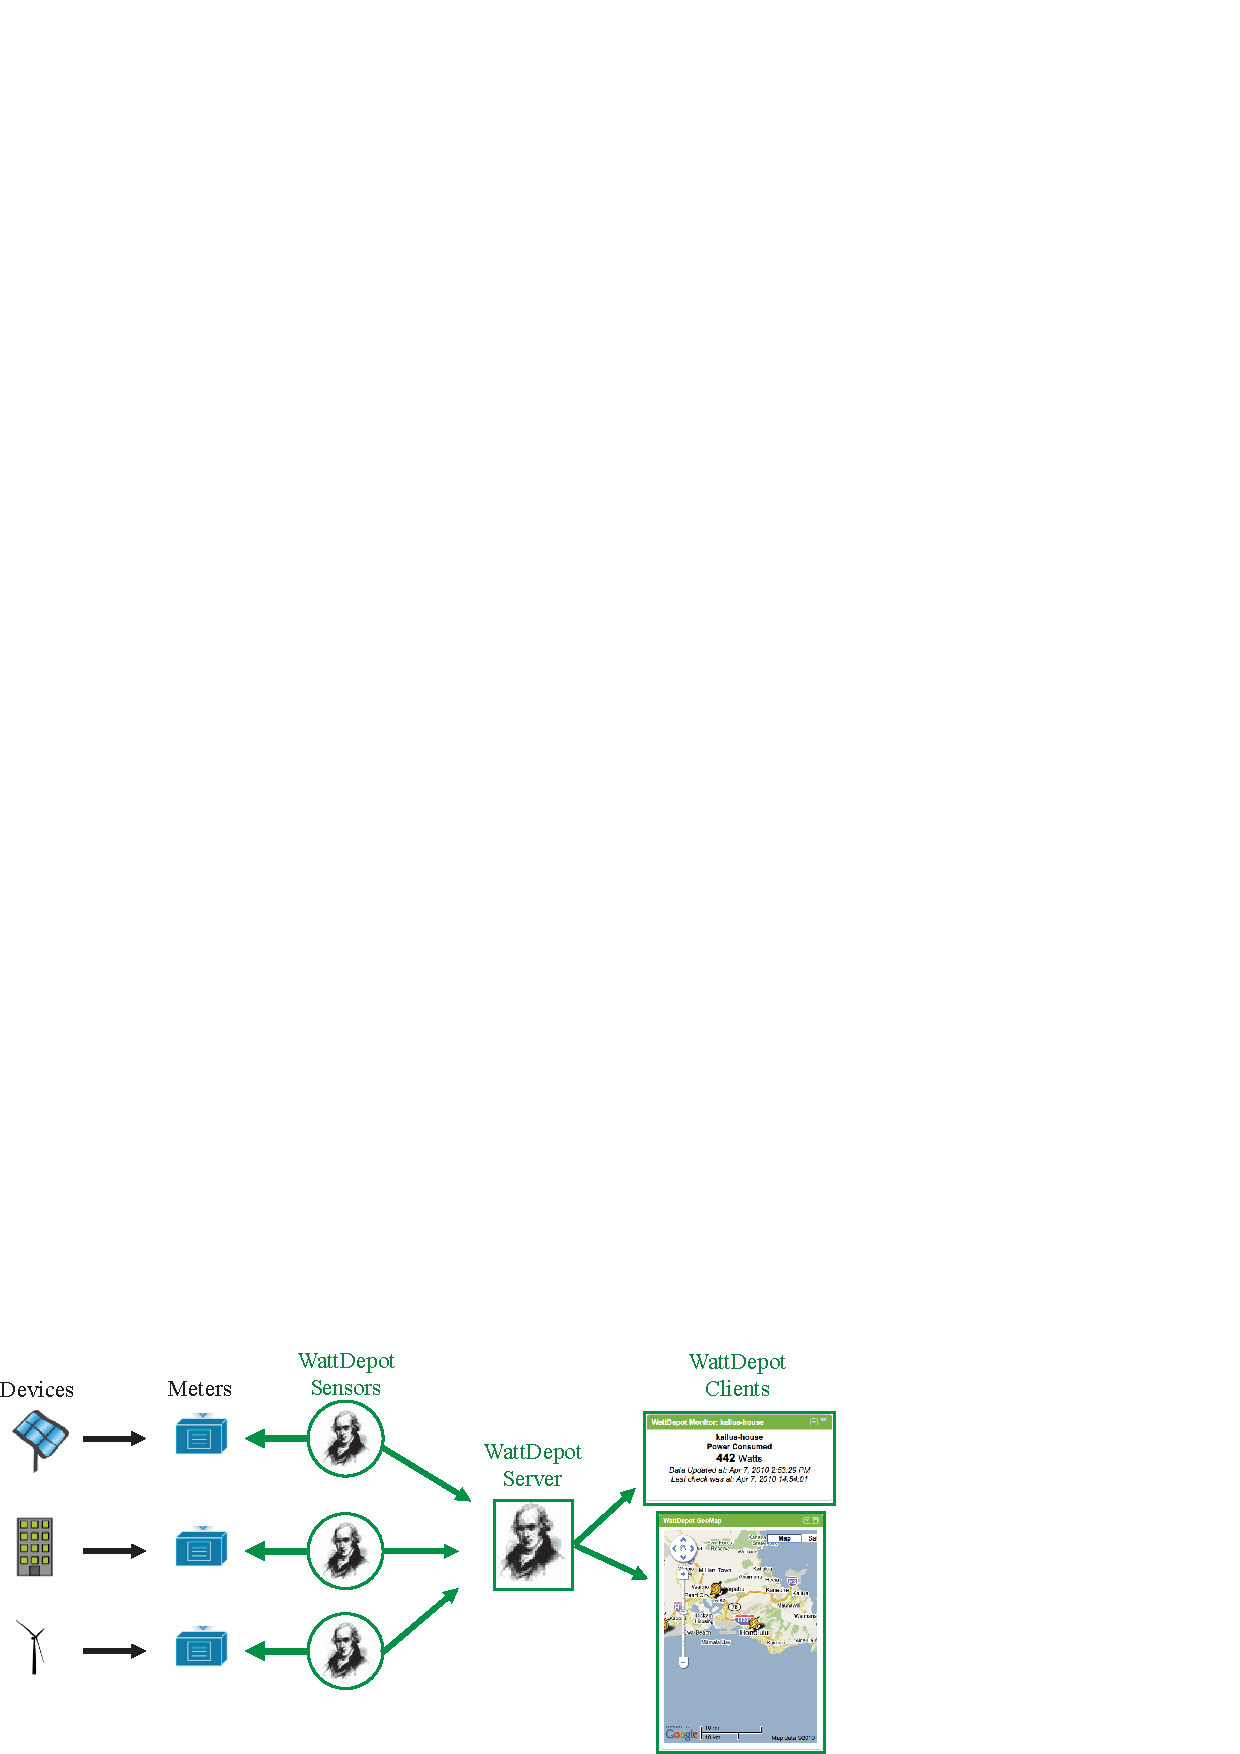
\includegraphics[width=\textwidth]{wattdepot-architecture}
		\caption{The architecture of the WattDepot system}
\label{fig:wattdepot-architecture}
\end{figure}

WattDepot is broken into three kinds of services:

\begin{enumerate}
\item WattDepot \emph{sensors}, a software process customized for a particular brand of energy meter, which requests data from a meter according to the meter's protocol, and then sends it to a WattDepot repository for storage;

\item WattDepot \emph{servers}, which implement a REST~\cite{REST} API for accepting energy data sent from sensors and providing this sensor data (or analyses based upon the data) to WattDepot clients; and

\item WattDepot \emph{clients}, which request data from WattDepot servers and either display the data or analyses directly to users or provide the data to higher level energy services.
\end{enumerate}

Data retrieved by sensors is associated with a \emph{source} when stored in the server. Each physical meter is typically a source, but sources can also be virtual combinations of other sub-sources. For example, as discussed in \autoref{sec:electrical-infrastructure}, the electricity used by each lounge is provided by two different panels with separate meters. To view the total electricity use of the lounge, I created a virtual source with the two meters feeding that lounge as sub-sources.

Once the energy data has been stored in a WattDepot server, clients can query the server for the amount of energy used by a source between two arbitrary points in time. Since the sensor data is only retrieved periodically, in most cases the endpoints for an energy query will not precisely match the sensor data. To solve this problem, the WattDepot server will linearly interpolate between the two nearest sensor data values before returning data to a client.

To retrieve data from the Shark meters, I wrote a sensor that retrieves two values from the meter: the instantaneous power consumed and an energy counter that records how many watt-hours have flown through the meter since it was constructed. The meters were polled every 15 seconds before and during the challenge, and the resulting sensor data was stored in a WattDepot server. Both the sensors and server were installed on a Apple Xserve system housed in our research lab. The client use of the energy data is discussed in \autoref{sec:energy-data-integration}.


\section{Challenge Design}

The Kukui Cup challenge was designed to meet multiple needs. In order to be effective, the challenge needed to be interesting and engaging for the participants, or they would not be interested in participating. As a research project, the challenge also had to support the needs of our experimental design and data collection. In some cases, these two needs were in conflict, and I note those decisions in this section and in \autoref{cha:evaluation}.

The Kukui Cup consists of two different competitions: an energy conservation competition, and a point competition. This section explains the design of those two competitions, and other important game components.


\subsection{Rounds}

The 2011 Kukui Cup was structured into three week-long rounds:

\begin{itemize}
	\item Round 1: Monday October 17 to Sunday October 23;
	\item Round 2: Monday October 24 to Sunday October 30; and
	\item Overall Round: Monday October 31 to Sunday November 6.
\end{itemize}

Each round began at the start of the beginning day (12:00 AM) and ended at midnight on the end date. Each round had separate prizes. Rule changes typically took place at the start of a new round, such as the referral bonus (see \autoref{sec:referral-bonus}). In Round 2, the points earned and energy used in Round 1 were set aside so that each player and lounge started at zero. The goal of this point/energy reset was to encourage residents who did not participate initially to start participating in a later round without undue disadvantage. In fact, since some activities could be performed in either Round 1 or Round 2, a player starting in Round 2 had an advantage in winning Round 2, as they could accrue all those points to their Round 2 total. In the Overall Round, the score and energy totals from Round 1 and Round 2 are combined, as well as any points earned in the Overall Round.


\subsection{Energy Competition}
\label{sec:energy-competition}

The 2011 Kukui Cup energy competition had a straightforward goal: the lounge that uses the least electrical energy in the round wins. As discussed in \autoref{sec:electrical-infrastructure}, monitoring energy at anything other than the lounge level was infeasible, making the lounge the fundamental unit of the energy competition.

Most other building energy competitions (such as the Oberlin competition discussed in Section \ref{sec:dorm-energy-competitions}) do not use absolute energy use as the metric for success. Most competitions record energy data before the competition, and then average that data in some way to produce a baseline of energy usage for the unit of competition (e.g., floor, building). The metric of success is then defined as the team that reduced their energy use during the competition by the largest percentage compared to their baseline usage. As most competitions involve buildings of different sizes, construction dates, and occupancy levels, comparing to baseline usage is the only way to provide normalization between the teams.

Using percent energy reduction compared to a baseline as the success metric for a competition means that it is critical to determine the baselines accurately. As discussed in \autoref{sec:baseline-computation}, determining an accurate baseline is challenging and potentially error prone. Also, using a baseline opens the possibility of a team artificially inflating their energy usage during the baseline collection period to make it easier for that team to win the competition. In another potential scenario, one can imagine two teams before the competition starts: team A is very conscientious about energy use and has already taken many energy saving measures, while team B uses energy very wastefully and has taken no energy saving measures. Team A would find it difficult to achieve much reduction from their baseline energy use during the competition, while team B can take the all the easiest energy-saving measures and achieve substantial reductions compared to their high baseline.

Absolute energy makes sense as a success metric for our energy competition because all four of the Hale Aloha towers have very similar construction, and they are all close to full occupancy since the demand for on-campus housing outstrips supply. On the other hand, baselines were used for the Daily Energy Goal Game, described in \autoref{sec:energy-goal-game}, to ensure that the goals were achievable based on the lounge's past energy use.

Participants were able to track their lounge's performance in the energy competition through the scoreboard provided on the challenge website, as shown in \autoref{fig:energy-scoreboard}.

\begin{figure}[htbp]
	\centering
		\includegraphics[scale=0.6]{round-1-energy-scoreboard}
		\caption{Round 1 energy scoreboard}
\label{fig:energy-scoreboard}
\end{figure}

We provided information to lounges on how to reduce their energy consumption through the activities and events available through the point competition.


\subsection{Point Competition}
\label{sec:point-competition}

In the point competition, individuals earned points by taking actions related to energy literacy or sustainability mediated through the challenge website. The points earned by individuals were also aggregated by lounge, to produce a score for each lounge.

One of the goals of the challenge was to improve the energy literacy of the participants. As discussed in \autoref{sec:energy-literacy}, I defined energy literacy as consisting of knowledge, skills, attitudes, and behaviors. While the knowledge component can be conveyed through information displayed on the challenge website, the behaviors require the participants to engage in activities outside the website. Further, research in environmental psychology described in \autoref{sec:fostering-behavior} indicates that the incorporation of techniques like public commitments can increase the likelihood of sustainable behavior change.

To increase the energy literacy of the participants and to motivate their participation, the website provides a variety of actions that participants can take. These actions are divided into three categories:

\begin{itemize}
	\item \emph{Activities:} one-time, verifiable actions
	\item \emph{Commitments:} ongoing, non-verifiable behaviors
	\item \emph{Events:} events scheduled at a particular place and time
\end{itemize}

The complete list of actions defined for the competition can be found in \autoref{app:actions}, and a summary of the actions can be seen in \autoref{tab:action-summary}.

\begin{table}[htbp]
	\centering
	\caption{Summary of the actions available during the challenge}
	\label{tab:action-summary}
	\vskip 1em
	\begin{tabular}{| l | c |}
		\hline
		Action type & Number available \tabularnewline \hline \hline
		Activities & 62 \\
		Commitments & 21 \\
		Events & 24 \\ \hline
	\end{tabular}
\end{table}

Actions can be either locked or unlocked. An unlocked action can be completed by a participant, while a locked action is completely inaccessible to participants until it is unlocked. Actions may be initially unlocked, while some actions may require other pre-requisite actions to be completed first. Actions may also be locked until a certain date. In the 2011 Kukui Cup, the available actions were divided roughly into thirds, and only the first third was available in Round 1, with the the second third available in Round 2, and then all actions were unlocked in the Overall Round.

When a participant successfully completes an action, they earn points. The points are intended to reflect the difficulty of the action. \autoref{tab:point-rubric} shows a summary of the different point levels and what type of action they correspond to.

\begin{table}[htbp]
	\centering
	\caption{List of point categories for actions}
	\label{tab:point-rubric}
	\vskip 1em
	\begin{tabular}{| c | l | c |}
		\hline
		Point value & Type of action & Time commitment \tabularnewline \hline \hline
		5 & Tweet something or complete a commitment & 1--2 min \\ \hline
		10 & Watch tutorial video, slightly more involved activities & 5 min \\ \hline
		20 & Attend an event & 1--2 hours \\ \hline
		30 & Priority events or activities & 10--60 min \\ \hline
		5--50 & Creative activities (e.g., writing a letter to editor) & multiple hours \\ \hline
	\end{tabular}
\end{table}


\subsubsection{Social Bonus}

As discussed in \autoref{sec:energy-competition}, participants must work together to win the energy competition. Provide an incentive for participants to work together, some actions in the point competition were assigned a \emph{social bonus}. The social bonus was worth 5 or 10 points, and was applied only to actions where two or more participants could reasonably complete the action together such as attending an event or making a commitment. To obtain the social bonus, a participant submits the email address of another participant with whom they completed the action. If the participant corresponding to the email address provided has completed the action, then the social bonus requester receives the bonus points. The social bonus does not require reciprocation: participant A can list participant B for the social bonus, and receives points even if participant B lists another participant or no one for the social bonus. The social bonus is a deliberately simplistic indication of social interaction, because only an email address exchange is required. There is no verification that an action where the social bonus has been used was completed collaboratively. However, obtaining another's email address provides participants with an excuse to initiate contact regarding the challenge, and we felt it was sufficient justification for any point inflation that might result.


\subsubsection{Referral Bonus}
\label{sec:referral-bonus}

In an effort to increase participation in the challenge, in Round 2, we instituted a \emph{referral bonus} (the idea for the referral bonus was suggested by Jenna Amberg-Johnson). When a participant logs into the challenge website for the first time, as part of the first login process, they are asked to enter the UH email address of another participant if that other participant referred them to the challenge. Once the new participant earns 30 points in the challenge, then both the new participant and the existing participant are awarded 10 bonus points. New participants that successfully completed the first login process earned 25 points, so to earn the bonus, new participants had to complete at least one activity. There was no limit placed on the number of times a participant could be used as the referrer.


\subsubsection{Activities}
\label{sec:activities}

Activities are the most common type of action available to participants. Activities are one-time actions that can be verified through the challenge website. Example activities include:

\begin{itemize}
	\item Watch a short YouTube video about Power \& Energy,
	\item Replace an incandescent bulb with a compact fluorescent (CFL),
	\item Perform an energy audit of the participant's room, and
	\item Write a letter to the editor on a Kukui Cup topic.
\end{itemize}

Once the activity has been performed, the participant must verify the completion in order to receive points. Each activity uses one of these four methods of verification:

\begin{itemize}
	\item A short answer to a question randomly selected from a list,
	\item An uploaded image (often a digital photo),
	\item An open-ended response in text, and 
	\item An open-ended response in text paired with an uploaded image.
\end{itemize}

In each case, the participant enters their verification information, which is sent to a challenge administrator for review. The administrator either approves the submission, at which point the participant receives their points, or rejects the submission with an informative message that explains why the submission was rejected. When a submission is rejected, the participant can try again, taking into account the administrator's reply. The review process happens asynchronously, so participants do not immediately know if their submission has been accepted. However, any submission does count as completing the action, so other actions that depend on the action submitted are unlocked.

As an example of the verification process, the video activities where the user watched a short video about an energy or sustainability topic used the short answer verification type. Each video had several verification questions, and to make it more difficult for participants to cheat by sharing answers, the question posed to each participant was selected randomly.

Other activities are difficult to verify with text only (such as changing out a incandescent bulb with a CFL). For these activities, participants can take a picture that provides some proof that they have completed the activity (such as holding both the incandescent bulb and the CFL).

The open-ended response verification type was used for activities where output of the activity was text, such as the letter to the editor activity. The open-ended response could also be used for activities where the result was a URL to a resource, such as a participant-created video.


\subsubsection{Commitments}
\label{sec:commitments}

Commitments are intentions to behave in a certain way in the future. The commitments in the Kukui Cup are intended to either improve participants energy literacy or reduce energy consumption, but for practical reasons cannot be verified through the website as activities are (see \autoref{sec:activities}). Example commitments are:

\begin{itemize}
	\item Turning off the lights when leaving a room,
	\item Turning off/shutting down all appliances before going to sleep, and
	\item Using sunlight instead of electric lighting.
\end{itemize}

While each of these commitments should reduce energy use, verifying compliance would require a massive network of embedded sensors throughout the towers, with a consequent massive invasion of participant privacy. The inability to verify that commitments are being met could lead participants to cheat and make commitments that they had no intention of meeting, just to earn points. We addressed this issue in two ways. First, commitments made by participants are public to all members of the same lounge. By making them public, we hope to encourage peers to point out commitments that have been made but are being violated. As discussed in \autoref{sec:rl-commitments}, public commitments have been shown to be more effective than private commitments, providing further reason to make commitments public. Second, each commitment is only worth 5 points (with a possible 5 point social bonus), each participant can only make five commitments at a time, and each commitment lasts for five days. Since the challenge lasts 21 days, this cap limits the number of points that a participant can earn from commitments at 200 points, which is low enough that a cheating participant (who commits with no intention of acting on the commitment) would not sabotage the point competition.

When a participant has made a commitment, they can return to the challenge website in five days to collect their points. The participant verifies their completion of the commitment by clicking on a button to affirm that they did live up to the commitment. While this self-verification still allows a participant to receive points without actually performing the commitment, it requires the participant to make a conscious decision to do so. Participants can repeat commitments after they expire, if they wish.


\subsubsection{Events}
\label{sec:events}

We held 24 events and excursions as part of the challenge. Events were generally workshops, games, or parties held on the UH \Manoa campus, while excursions took place off-campus. Some examples of events are:

\begin{itemize}
	\item Kickoff party (held on evening of first day of challenge),
	\item Energy scavenger hunt (looking for devices using specific amounts of power), and
	\item Wind farm tour.
\end{itemize}

Participants could view the list of upcoming events on the challenge website, and could sign up to indicate their desire to attend. Signing up for an event earned participants 2 points instantly. To verify attendance, at each event a challenge administrator handed out small printed slips of paper that contain an \emph{attendance code}. Each attendance code is unique to the event, and contains a random string of characters generated by the website in advance, such as {\tt windfarm-it397}. After the event is complete, participants that attended can enter the attendance code they received into the challenge website. The website then verifies that the code is valid, has not already been used, and corresponds to the event in question. Unlike activity verification, if the code is valid, the participant is awarded points immediately upon submission. To encourage participants to only sign up for events they actually wanted to attend, participants that signed up for an event but failed to enter an attendance code (either because they did not attend the event or they forgot to enter the code) were penalized 4 points: reversing the 2 point signup bonus and deducting a 2 point penalty.


\subsection{Daily Energy Goal Game}
\label{sec:energy-goal-game}

As described in \autoref{sec:goals}, setting goals for energy conservation has been shown to aid in conservation efforts. To help lounges reduce their energy use, we created the Daily Energy Goal Game, where each lounge attempts to use less energy each day than the goal set. The goal was determined by computing a baseline of energy use for each lounge and subtracting a fixed percentage from each baseline. At the end of each day, if a lounge had met its energy goal, each resident in the lounge who is participating received 20 points.

The Daily Energy Goal Game had two additional benefits for the challenge design. First, it provided a short-term energy goal that participants could work towards, shortening the feedback cycle. If a lounge failed to meet the goal one day, the participants could redouble their efforts and try again the next day. Second, it provided a further linking of the energy competition to the point competition.

To aid participants in meeting their daily goal, the challenge website provided a visualization of progress towards the goal, shown in \autoref{fig:energy-goal-game}.

\begin{figure}[htbp]
	\centering
		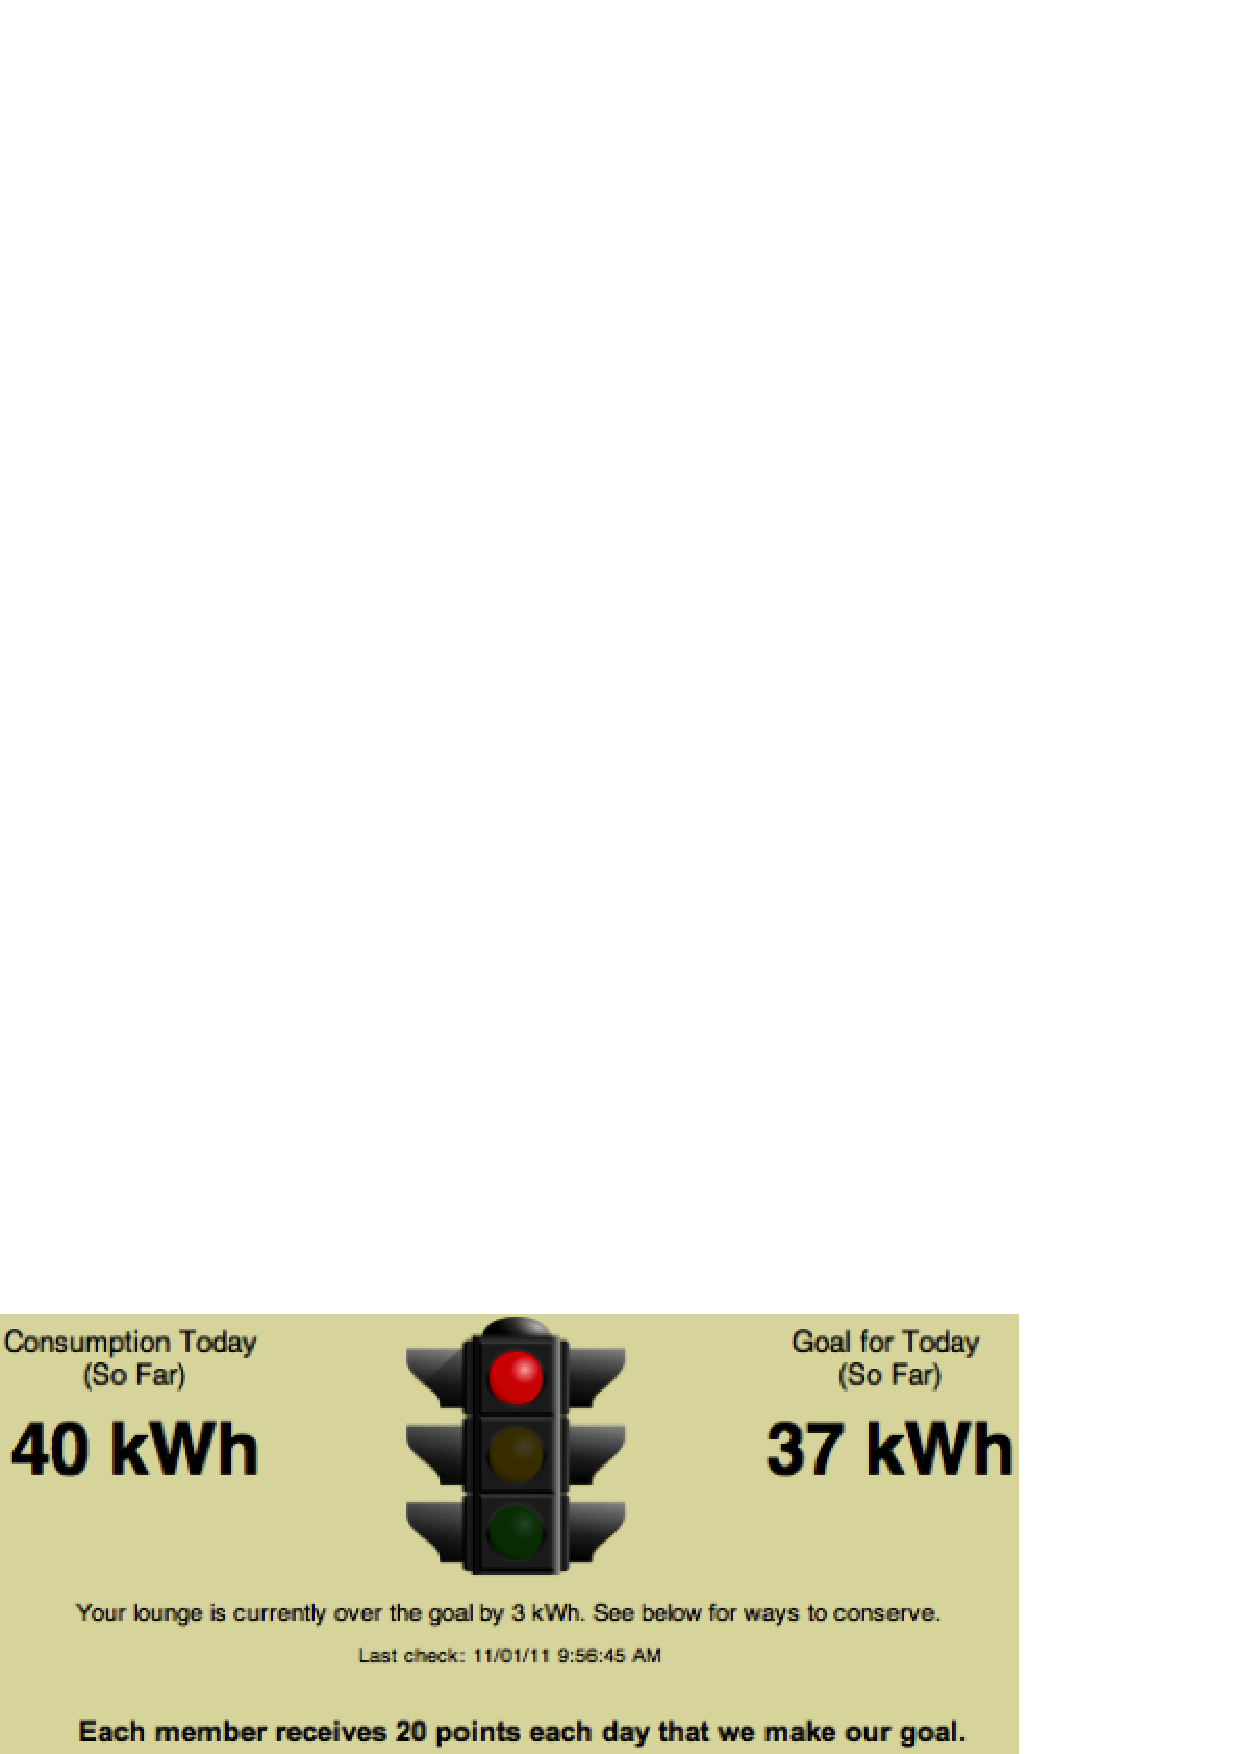
\includegraphics[scale=0.7]{energy-goal-game}
		\caption{Example of the Daily Energy Goal Game visualization}
\label{fig:energy-goal-game}
\end{figure}

We computed the baseline of each lounge's energy use on an hourly basis. The visualization shows the number of kilowatt-hours used by the lounge so far in the day, and compares it to the energy use goal. The traffic light indicates the energy use: red, when the energy use is above the goal; yellow, when energy use is just below the goal; and green, when energy use is significantly below the goal. Both yellow and green thresholds are configurable.

It was important that the visualization compare the energy use for the day so far, to an equivalent goal for the day so far. Since cumulative energy use is monotonically increasing, if the energy use were compared to the goal for the entire day, it would generally lead to a traffic light that is green for part of the day and then stays red for the rest of the day, which would not be an actionable visualization for participants. Further, we computed the baselines at an hourly granularity, because energy use varies throughout the day. Not doing so, i.e., computing a single daily baseline value and averaging it throughout the day, would cause the visualization to show participants under the goal during the low usage period of the day, but then over the goal during the evening high use period.


\subsubsection{Baseline and Goal Computation}
\label{sec:baseline-computation}

The energy goal for the Daily Energy Goal game requires a baseline of energy use for each lounge. The baseline should reflect ``normal'' use, and be closely comparable to the energy use during the challenge period. \autoref{fig:lounge-daily-power} shows the power used by one lounge over the course of a weekday before the challenge, while \autoref{fig:lounge-weekly-power} shows the power used by the same lounge over an entire week. The energy use for the lounge differs from an average home or apartment in a few ways: the peak power usage is shifted to near midnight for weekdays, the lowest usage occurs between 8 AM and 10 AM which is typically a high usage period in homes. Usage also varies based on the day of the week: Friday and Saturday evenings have lower and earlier peaks compared to other nights. To capture these hourly and daily variations, we computed baselines each of the days of the week (seven daily baselines), and for each hour of each day of the week (i.e., 168 hourly baselines).

\begin{figure}[htbp]
	\centering
		\includegraphics[width=\textwidth]{Ilima-B-daily-power}
		\caption{Example power usage by Ilima B for one day, pre-challenge}
\label{fig:lounge-daily-power}
\end{figure}

\begin{figure}[htbp]
	\centering
		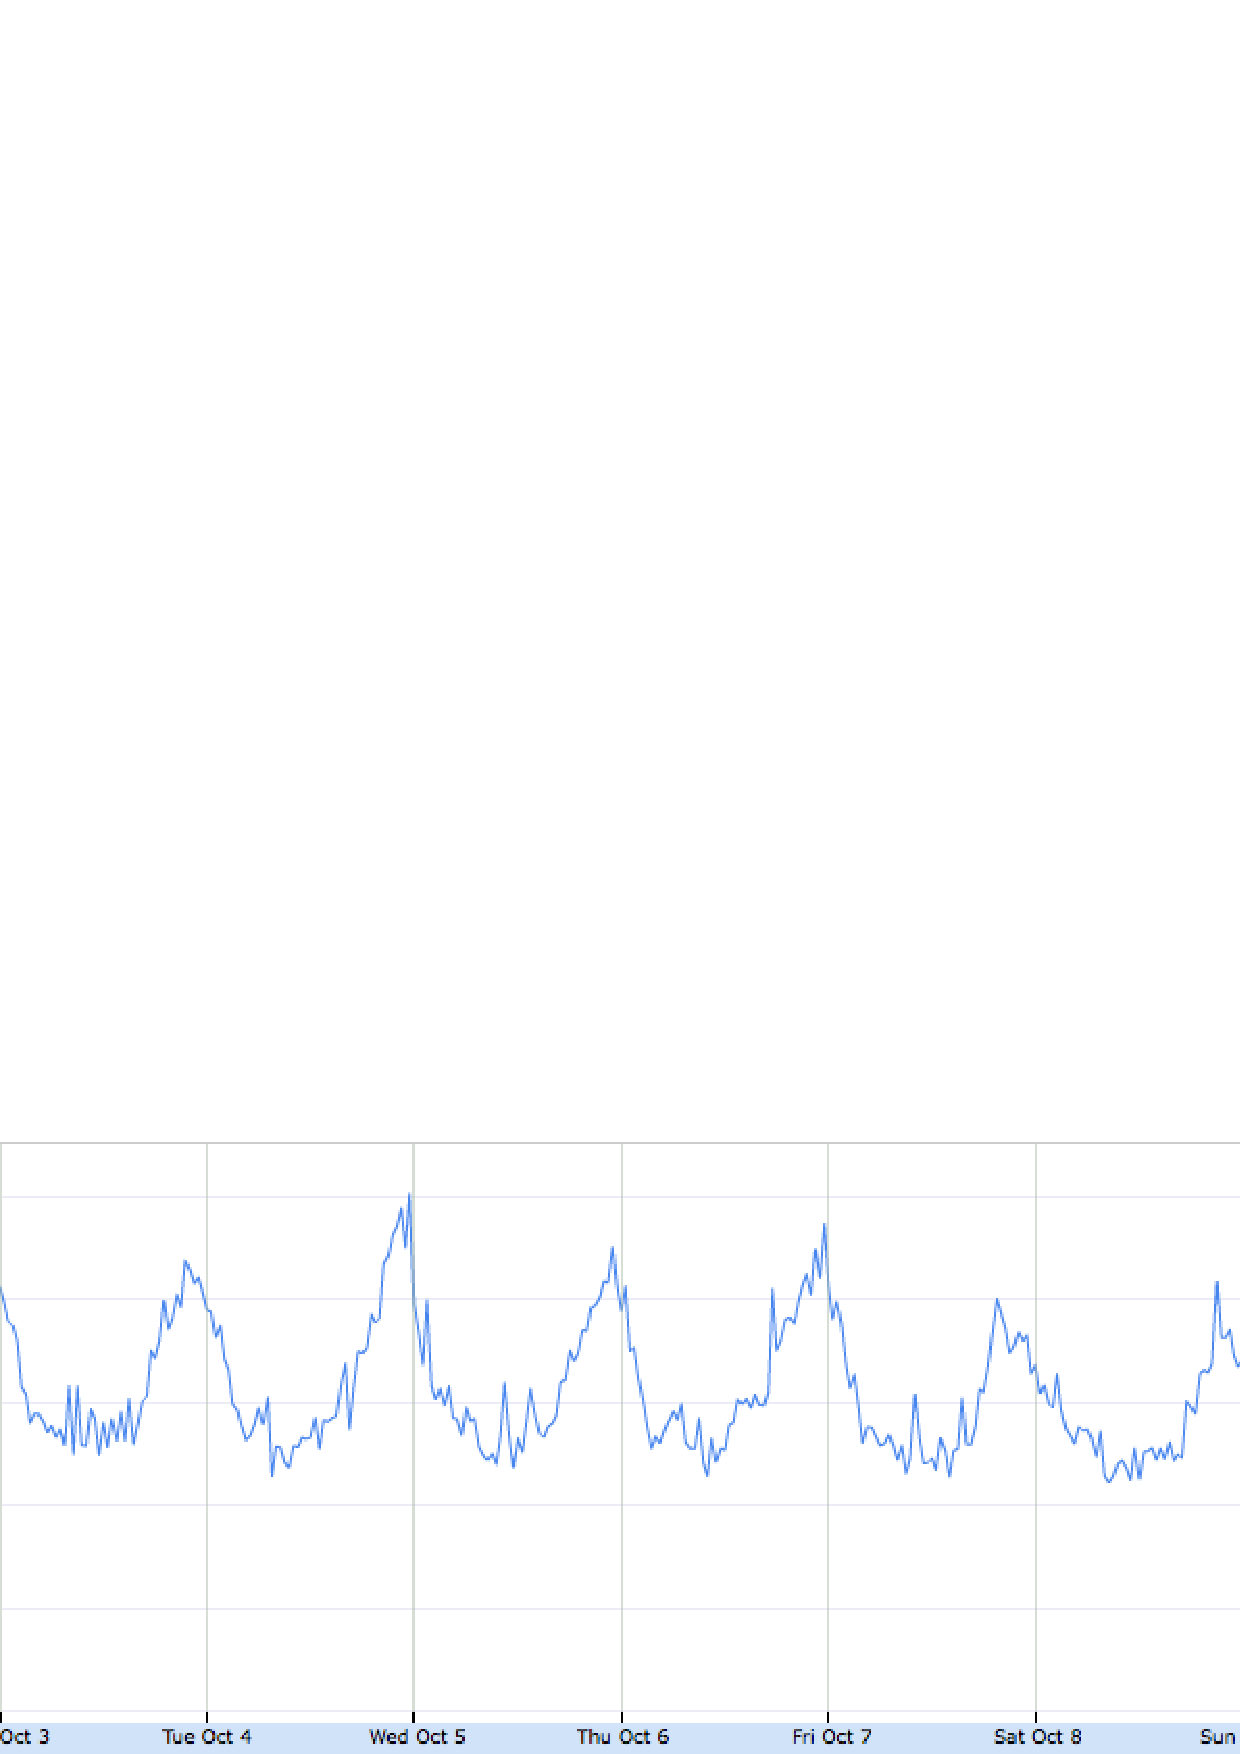
\includegraphics[width=\textwidth]{Ilima-B-weekly-power}
		\caption[Example power usage by Ilima B for one week, pre-challenge]{Example power usage by Ilima B for one week, pre-challenge. Dates on x-axis indicate the start of that day (i.e., midnight).}
		\fxnote{Replace with publication-quality graphs if time permits}
\label{fig:lounge-weekly-power}
\end{figure}

The challenge ran for three weeks starting October 17, 2011. As shown in \autoref{tab:meter-timeline}, full days of meter data for all lounges were only available for Lehua, Ilima, and Mokihana starting on September 10. For lounges in these three towers, I computed the initial baseline as the average energy use from September 10 to October 15 (five full weeks plus one day). The delay in getting meters installed and working properly in Lokelani complicated the baseline computations for that tower. Lokelani A and E got their first full day of data on October 7, so the baseline was computed from October 7 to October 15 (one full week and two days). The baseline for the days of the week with two days of data are were averaged, the rest reflect the actual usage.

The late installation of the meters in Lokelani B, C, and D meant that I had less than one week of data for those lounges before the challenge began. I felt that it was important from a challenge perspective for all lounges to be able to participate fully in the challenge, rather than exclude Lokelani B, C, and D from participating in the the Daily Energy Goal Game or the entire challenge. Lokelani C and D had data from Wednesday October 12 to Saturday October 15, so I used the actual usage as the baseline for those days of the week. For the remaining two weekdays (Monday and Tuesday), I computed the baseline by averaging the data from the three weekdays. Usage on Sunday is different from both weekday and Saturday usage, requiring some additional calculation to provide a reasonable estimate. I computed the ratio of energy use between Sunday and Saturday for each lounges in Lehua, Ilima, Mokihana, and Lokelani A and E. I found the average increase in daily energy use from Saturday to Sunday from the baseline period is 5\%, so the Sunday value for Lokelani C and D was the actual usage from Saturday October 15 multiplied by 1.05.

Lokelani B presented the biggest challenge in estimating an energy baseline, since I had only one full day of data from Saturday October 15. I assumed (for lack of other alternative) that the ratio of energy use between lounges on a single day is representative of the ratio of their energy use for each day of the week. For the weekday values, I computed the ratio of energy use on October 15 between Lokelani A and B, and between Lokelani B and E, since lounges A and E were in the same tower and had more than a full week of data. I set the baseline for each weekday as the average of the A to B ratio multiplied by the A  baseline for that day, and the B to E ratio multiplied by the E baseline for that day.
%\fxnote{Need series of plots showing energy use before challenge, and then the 1 week baseline}

Because of the limited energy data for Lokelani, the baselines for Lokelani were speculative extrapolations. However, as discussed earlier in \autoref{sec:energy-baselines}, I was using the baselines here as part of a game mechanic to spur conservation, rather than as a way of evaluating the challenge.


\subsection{Energy Goal and Baseline Changes}

The energy goal for the Daily Energy Goal Game was initially set to a 5\% reduction in energy use compared to the lounge's baseline energy use. On the first day of the challenge, 5 of the 20 lounges had already met the 5\% daily energy reduction goal. Since the challenge had only been running for 24 hours, with the Kickoff Party event taking place at 6:30 PM, we felt it was unlikely that the challenge could have caused the change. Therefore, it seemed likely that those lounges made their goal due to random variations in energy use rather than behavioral change. For this reason, we set the daily energy goal to 10\% for the remainder of Round 1 of the challenge.

Due to the problems we encountered in setting initial baselines for energy use in the lounges, in the interests of fairness, we decided that the baselines should be recomputed for Round 2. We recomputed the baselines for each lounge based on each lounge's energy use during Round 1, ensuring that the baselines were computed with a whole week of data for each lounge. For lounges that had reduced their energy use in Round 1, the new baseline had the side effect of making it harder to meet the goal, since the new baseline would be lower than the initial one. To compensate for the added difficulty, we changed the daily energy goal percentage back to 5\%. We used the new baseline and goal percentage unmodified in the final round of the challenge.


\subsection{Prizes}
\label{sec:prizes}

Prizes were awarded at the end of each round as incentives for participation. There were four categories of awards:

\begin{itemize}
	\item The lounge that used the least energy (1 winner per round),
	\item The lounge with the highest score (1 winner per round),
	\item The individual with the highest score in each lounge (20 winners per round), and
	\item The individual with the highest score across all lounges (1 winner per round).
\end{itemize}

In Round 1 and Round 2, only the score earned or energy consumed for that round was used to determine the winner. In the third round, called the Overall Round, however, the overall score or energy was used. There were no prizes awarded just for scores from the third round. \autoref{tab:prizes} summarizes the prizes awarded during the challenge. As one would expect, the prizes for the Overall Round (the third and final round) were substantially higher value than the prizes for Rounds 1 and 2.

\begin{table}[htbp]
	\centering
	\caption{Prizes awarded during challenge}
	\label{tab:prizes}
	\vskip 1em
	\begin{tabular}{| c | l | l |}
		\hline
		Round & Type of prize & Prize \tabularnewline \hline \hline
		1 & lounge energy & mochi ice cream party \\ \hline
		1 & lounge score & cupcake party \\ \hline
		1 & individual per lounge & \$5 ice cream gift certificate \\ \hline
		1 & individual overall & \$25 UH bookstore gift certificate \\ \hline
		2 & lounge energy & malasada party \\ \hline
		2 & lounge score & locally-made popsicle party \\ \hline
		2 & individual per lounge & \$5 gelato gift card \\ \hline
		2 & individual overall & \$25 UH food service gift card \\ \hline
		overall & lounge energy & pizza party \\ \hline
		overall & lounge score & pizza party \\ \hline
		overall & individual per lounge & \$10 UH bookstore gift card \\ \hline
		overall & individual overall & iPad 2 \\ \hline
	\end{tabular}
\end{table}


\subsection{Raffle Game}
\label{sec:raffle-game}

One problem with the prizes provided in the challenge as incentives is that they only go to the top performers in each competition. For those participants who are aware that they will not win the point competitions, the prizes provide little incentive, or possibly a disincentive: why play if there is no way to win a prize? Another problem with the prizes is that to be effective, they had to appeal to all participants, limiting the options for prizes.

We developed the Raffle Game to provide a prize-based incentive to play that was not limited to the top players, through inspiration from Balaji Prabhakar's work incentivizing road congestion reduction~\cite{Merugu2009}. In the Raffle Game, there are a variety of raffle prizes available in each round of the challenge. For each 25 points a participant earns, they receive a virtual raffle ticket. Participants can allocate their raffle tickets among the prizes available, and they can change their allocations at any time. Shortly before the end of the round, the raffle is closed and the ticket allocations frozen. A winning ticket is ``drawn'' from those allocated to each raffle prize, and the owner of that ticket wins the prize. Tickets that are not allocated before the end of a round roll over to the next round, until the end of the challenge. \autoref{fig:raffle-game} shows an example view of the Raffle Game for a user with many tickets, including the odds of winning.

\begin{figure}[htbp]
	\centering
		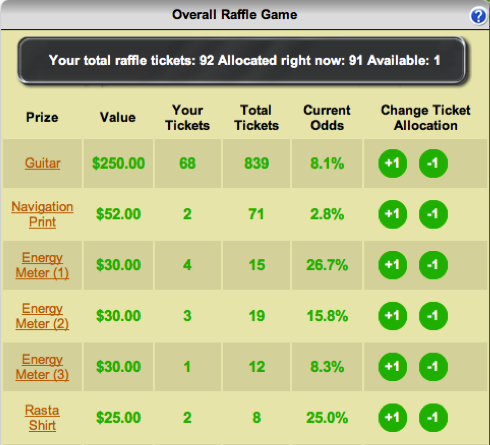
\includegraphics[scale=1.0]{raffle}
		\caption{Example display of the Raffle Game during the Overall Round}
\label{fig:raffle-game}
\end{figure}

The Raffle Game ensured that every participant who has earned at least 25 points in a round can have some slim chance of winning a prize. Participants can increase their odds of winning a prize by earning more points, providing a clear incentive for further participation. Because participants can choose which raffle prizes to allocate their tickets to, the prizes can appeal to diverse interests, unlike the competition prizes.

\section{Challenge Website}
\label{sec:challenge-website}

The Kukui Cup challenge required extensive online support for both the virtual and real-world activities. We developed a custom web application called Makahiki to be the online focus for the challenge. I was one of the principle designers of the functionality of the website, while application was implemented by George Lee, Yongwen Xu, with assistance from Greg Burgess, Nathan Dorman, and Nathaniel Ashe. The application is written in Python, using the Django web application framework~\cite{django-website}.

\subsection{Website Development}

The website was developed in an iterative fashion. An initial version was developed in Fall 2010 with limited input from anyone outside the development team. After showing this alpha version of the website to some external individuals, we received feedback that the website was too confusing and not sufficiently engaging.

Our next step was to develop a series of user scenarios, and visualize them using mockup web pages developed with Balsamiq Mockups tool~\cite{balsamiq-website}. The mockups were evaluated by a series of walkthroughs conducted with three UHM ICS faculty members, two community members, and two undergraduate students. Each evaluation was conducted using a think aloud protocol, as the participants viewed each mockup screen on a projector, while the experimenter walked through each user scenario. We recorded the discussion between the participant and experimenter, as well as the computer display. After the evaluations, we revised the mockups based on the feedback we had received.

In Spring 2011, Makahiki was implemented using the revised mockups as the template. In April 2011, we conducted a series of in-lab user evaluations of the website using five first-year students who were living in the Hale Aloha towers. We told the participants that the website they were evaluating was part of an energy challenge we were going to hold in the Fall 2011. We provided no additional details, because one important goal of the challenge website was to be self-explanatory. In the first part of the evaluation session, each participant was asked to pretend they were participating in the challenge, using a think aloud protocol. Participants interactions with the website were recorded as a screencast, along with audio from their interactions with the experimenter. In the second part of the evaluation, the experimenter went over parts of the website with the participant, while asking them questions about their experiences. After reviewing the comments from all five participants, we generated a list of improvements to be made to Makahiki.

In July 2011, once the problems identified with Makahiki from the April evaluation had been resolved, we conducted another round of in-lab user evaluations with five more participants. This evaluation was conducted in similar fashion, with participants pretending to be participants in the challenge and using the website while their actions and discussion was recorded. These evaluations resulted in another set of improvements in Makahiki.

While the in-lab evaluations were helpful, each one involved less than one hour of play, and the website designers were at hand to answer any questions in person. Since we conducted the in-lab evaluations individually, they didn't provide any insight into the competitive aspects of the Kukui Cup. To address this gap in our evaluation, we organized a beta test of the Kukui Cup in August 2011. We recruited four teams of five players, from friends, family, colleagues from industry, and local environmental organizations. The beta test consisted of two three day rounds to allow us to test the awarding prizes and the Raffle Game. The beta test uncovered several implementation defects that were corrected, as well as suggestions for additional actions. Further details on the development of Makahiki can be found in George Lee's thesis~\cite{csdl2-11-01}.


\subsection{Website Functionality}

We designed the challenge website to be as easy as possible for residents to start participating. This section describes the features of the website.


\subsubsection{First Login Process}
\label{sec:first-login}

During the challenge, when users went to the website~\cite{kukuicup-website}, they saw a landing page like the one shown in \autoref{fig:landing-page}. The landing page guides the residents eligible to play (those living in Hale Aloha) into the challenge site, while providing some background information on the challenge for everyone else.

\begin{figure}[htbp]
	\centering
		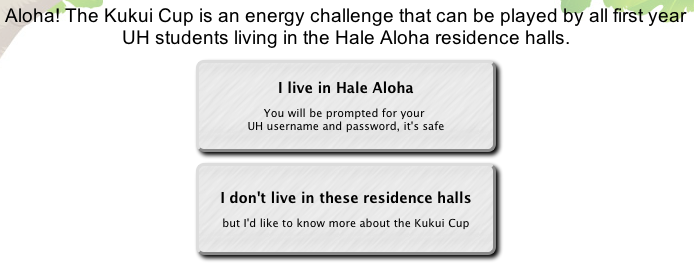
\includegraphics[scale=0.6]{landing-page}
		\caption{A portion of the challenge website landing page}
\label{fig:landing-page}
\end{figure}

To provide each participant with personalized information, the challenge website required participants to log on with their University of \Hawaii username and password. Using their existing credentials ensured that participants did not have to remember another username and password, which could have been a barrier to participation. The integration was made possible using UH's Central Authentication System. Using a roster provided by UH Student Housing, we were able to prepare accounts for all residents, including which lounge they were living in.

The initial experience of bringing a new player into a game is referred to as \emph{onboarding}~\cite{zichermann2011gamification}. This process is critical, because all players will experience it, and if the onboarding experience is poor, then potential participants may never sign up or play the game. In our user evaluations, we found that the onboarding process needed to explain the basic mechanics of the game, but remain short enough that new players would complete the process.

After logging in, new participants were sent through a first-login process. There were seven steps in the process:

\begin{enumerate}
	\item Introduction and chance to verify tower and lounge residence;
	\item Terms and conditions, including informed consent;
	\item Referral bonus email address entry (see \autoref{sec:referral-bonus});
	\item Profile setup, choosing display name, profile picture;
	\item Introductory video, a 2:09 long embedded YouTube video;
	\item Question based on introductory video; and
	\item Completion of first-login process.
\end{enumerate}


\subsubsection{General Page Structure}

After the first-login process is complete, and on each subsequent log-on, participants were taken to the home page as shown in \autoref{fig:home-page}. The header of the page is shared across all pages on the website. On the left side of the header is the Info Bar, which shows how many points the participant has earned, their standing in the competition, and energy use by their lounge. The Info Bar rotates through the different displays every few seconds. On the right side of the header is the Navigation Bar that contains icons representing the six pages in the website: clicking on the icon takes the user to that page.

\begin{figure}[htbp]
	\centering
		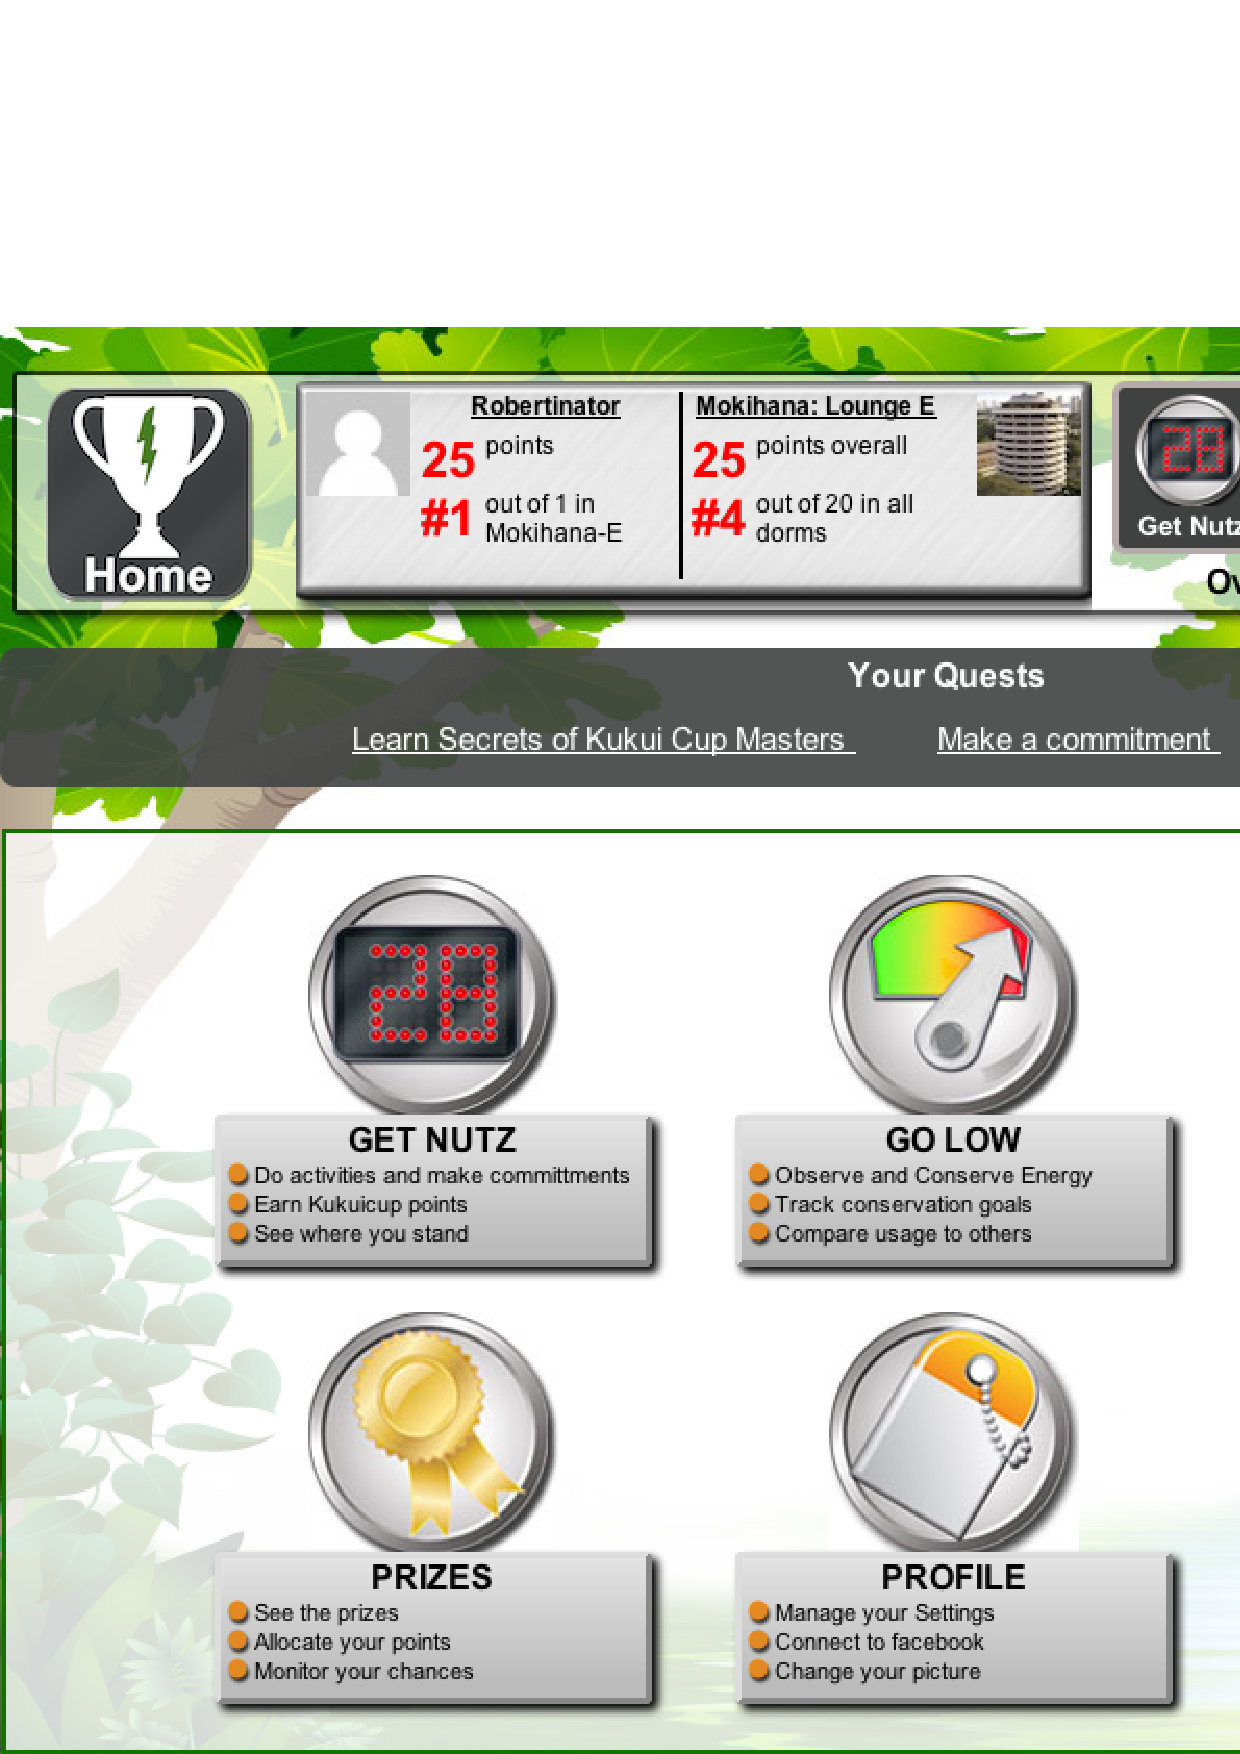
\includegraphics[width=\textwidth]{home-page}
		\caption{The challenge website home page}
\label{fig:home-page}
\end{figure}

Below the header is the Quest Bar, which shows the quests available to the participant. We created quests to guide participants through the website and the actions they could take. Each quest has a name, a description, a level, unlock conditions, and completion conditions. The up to three unlocked quests were shown  to participant in the quest bar, ordered by the level of the quest from lowest to highest. If the participant clicked on a quest title, the quest bar expands to show the quest description. After seeing the quest description, participants can choose to accept the quest or close the quest description. Once accepted, the quest is active until the participant meets the completion conditions. Some example quests from the 2011 Kukui Cup were:

\begin{itemize}
	\item ``Learn Secrets of Kukui Cup Masters'', which required participants to watch a video explaining some tips on how best to play the Kukui Cup.
	\item ``Sign up for an event'', which guided participants through the process of signing up to attend their first event.
	\item ``Get the Fully Committed Badge'', which encourages participants to sign up for five commitments, thereby earning the badge.
\end{itemize}

The six pages of the site are:
\begin{itemize}
	\item Get Nutz: take actions for points, view scoreboards;
	\item Go Low: real-time energy data, Daily Energy Goal game, energy; scoreboard
	\item News: shared lounge ``wall'' (like Facebook) with recent actions taken and discussion;
	\item Prizes: list of prizes and Raffle Game;
	\item Profile: make changes to display name, view list of past actions taken;
	\item Help: rules of challenge, frequently asked questions; and
	\item Canopy: a special area of the site where advanced users can view additional energy visualizations
\end{itemize}

I now examine each of the pages in turn.


\subsubsection{Get Nutz Page}
\label{sec:get-nutz-page}

The Get Nutz page is the primary place where participants could engage in the point competition. The title of the page refers to the kukui nut that the Kukui Cup is named after. \autoref{fig:get-nutz} shows the a view of the Get Nutz page from the Overall Round of the challenge.

\begin{figure}[htbp]
	\centering
		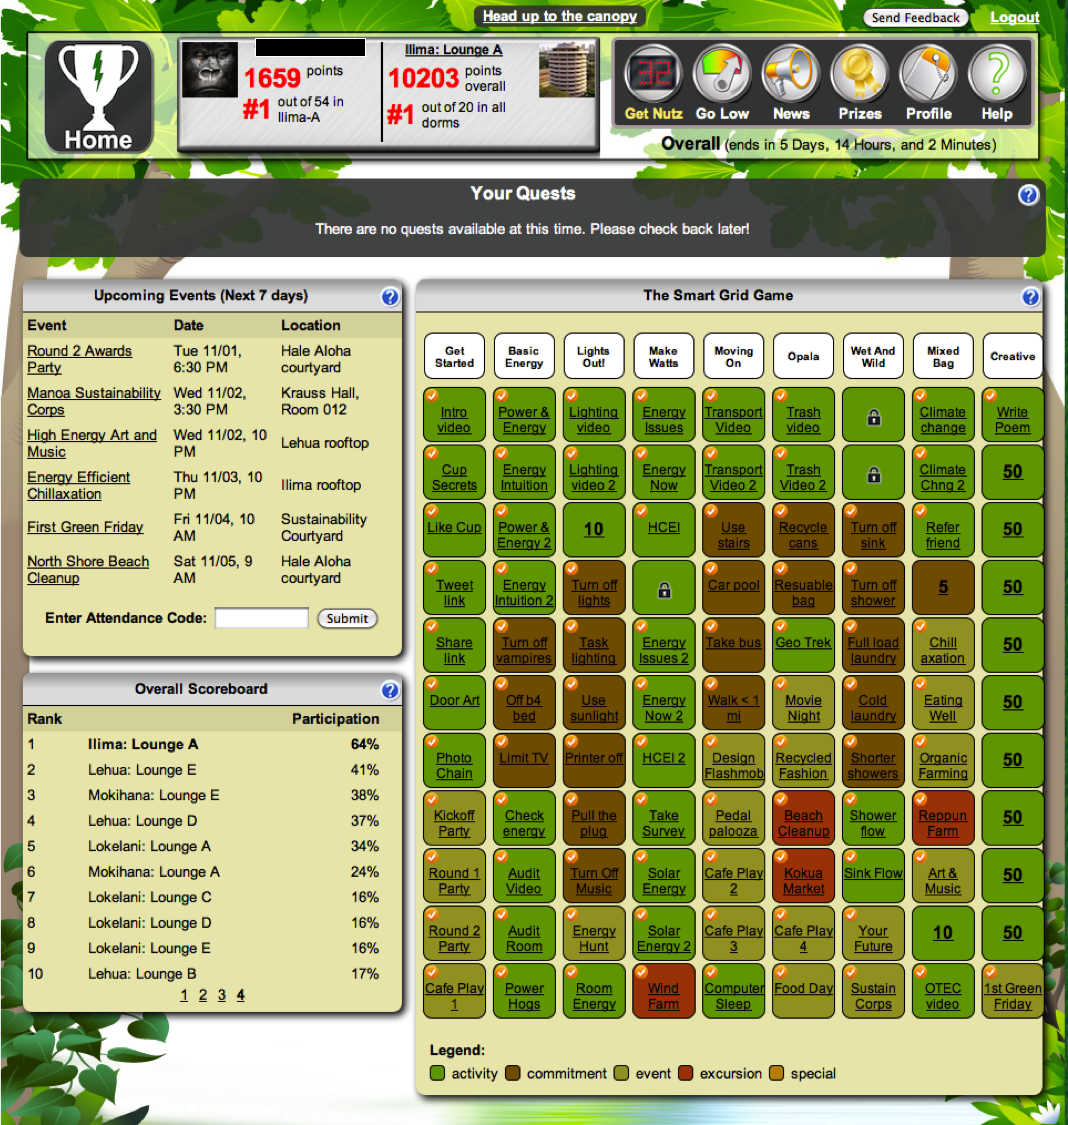
\includegraphics[width=\textwidth]{get-nutz}
		\caption{The Get Nutz point competition page}
\label{fig:get-nutz}
\end{figure}

The main focus of Get Nutz is the Smart Grid Game, which takes up most of the right side of the page. The Smart Grid Game organizes the actions described in \autoref{sec:point-competition} that participants can take to earn points. Each column organizes actions around a particular topic, such as ``Make Watts'' for actions related to energy generation. Each type of action had a different color. Actions that are unlocked display only the point value associated with the action, while locked actions are displayed with a lock icon. Once an action has been completed, the cell displays the name of the action and a small checkmark in the upper-left corner.

On the left side of Get Nutz are the Upcoming Events widget and the Scoreboard widget. Upcoming Events showed events that will take place over the next seven days. Each entry is a link to the event page, which displays details of the event and allows participants to sign up for the event. The Upcoming Events widget also allowed participants to type in event attendance codes directly, without navigating to the event details page.

The Scoreboard widget rotates through four separate scoreboards showing the top ten entries in different categories for the current round: lounge scores, individual scores across all lounges, individual scores within participant's lounge, and participation rates of lounges (see \autoref{sec:active-participation-bonus}).


\subsubsection{Go Low Page}
\label{sec:go-low-page}

The Go Low page is the focal point for the energy competition. The page is titled Go Low to remind participants that in the energy competition, the lowest energy use wins (unlike the point competition, where the goal is to obtain as many points as possible). \autoref{fig:go-low} shows a view of the Go Low page from the Overall Round of the challenge.

\begin{figure}[htbp]
	\centering
		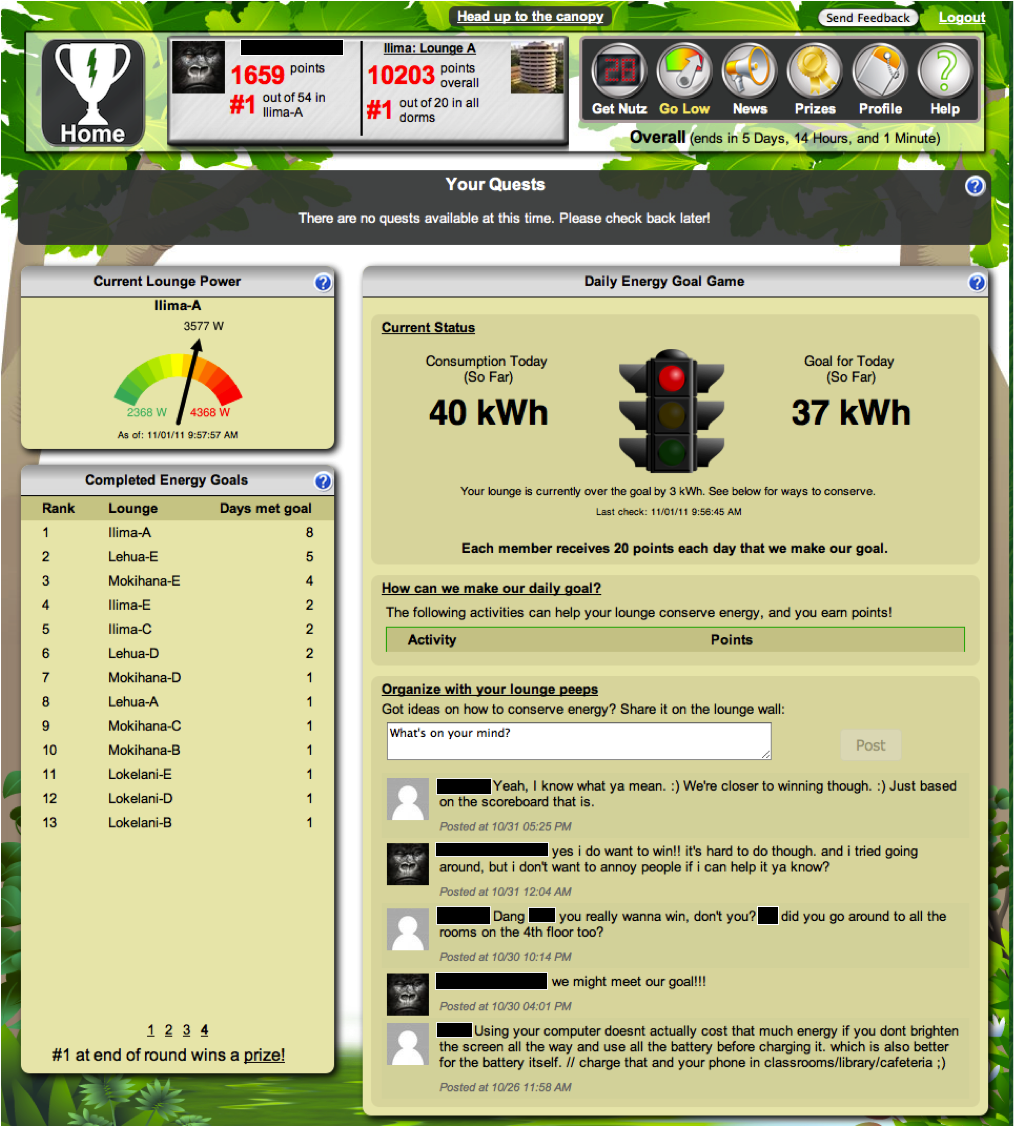
\includegraphics[width=\textwidth]{GoLow-round3}
		\caption{The Go Low energy challenge page}
\label{fig:go-low}
\end{figure}

The right side of the page shows the Daily Energy Goal game, described in \autoref{sec:energy-goal-game}. The visualization of the Daily Energy Goal game was implemented in JavaScript, so updates happen dynamically in the browser. To help participants meet their goal, below the Daily Energy Goal game is a section listing actions in the Smart Grid Game related to energy conservation (the list is empty in \autoref{fig:go-low} because the participant has completed all the relevant actions). The bottom portion of the right hand section contains the shared lounge discussion area, called the lounge \emph{wall} after the similar feature in Facebook. Participants can type short messages on the lounge wall that are displayed to all members of the lounge in reverse-chronological order. The wall is intended to provide a communication tool for the participants to strategize about energy conservation.

The left side of the page contains the Current Power widget and the Energy Scoreboard widget. The Current Power widget shows the power consumption of the participant's lounge, updated once every 15 seconds. The gauge is calibrated so that the needle pointing directly up corresponds to the average baseline power usage for the current hour of the day. When the needle moves to the right side of the gauge, it represents higher than average power usage for the current time of day, while the left side represents lower than average power usage. The gauge was implemented in JavaScript using the Google Visualization API.

The Energy Scoreboard widget ranks all twenty lounges in order of increasing energy use for the current round, and all previous rounds. It also shows a ranking of lounges by the number of energy goals completed by the lounge.


\subsubsection{News Page}
\label{sec:news-page}

The News page of the challenge website showed participants what was happening in the challenge and in their lounge. \autoref{fig:news-page} shows an example of the News page.

\begin{figure}[htbp]
	\centering
		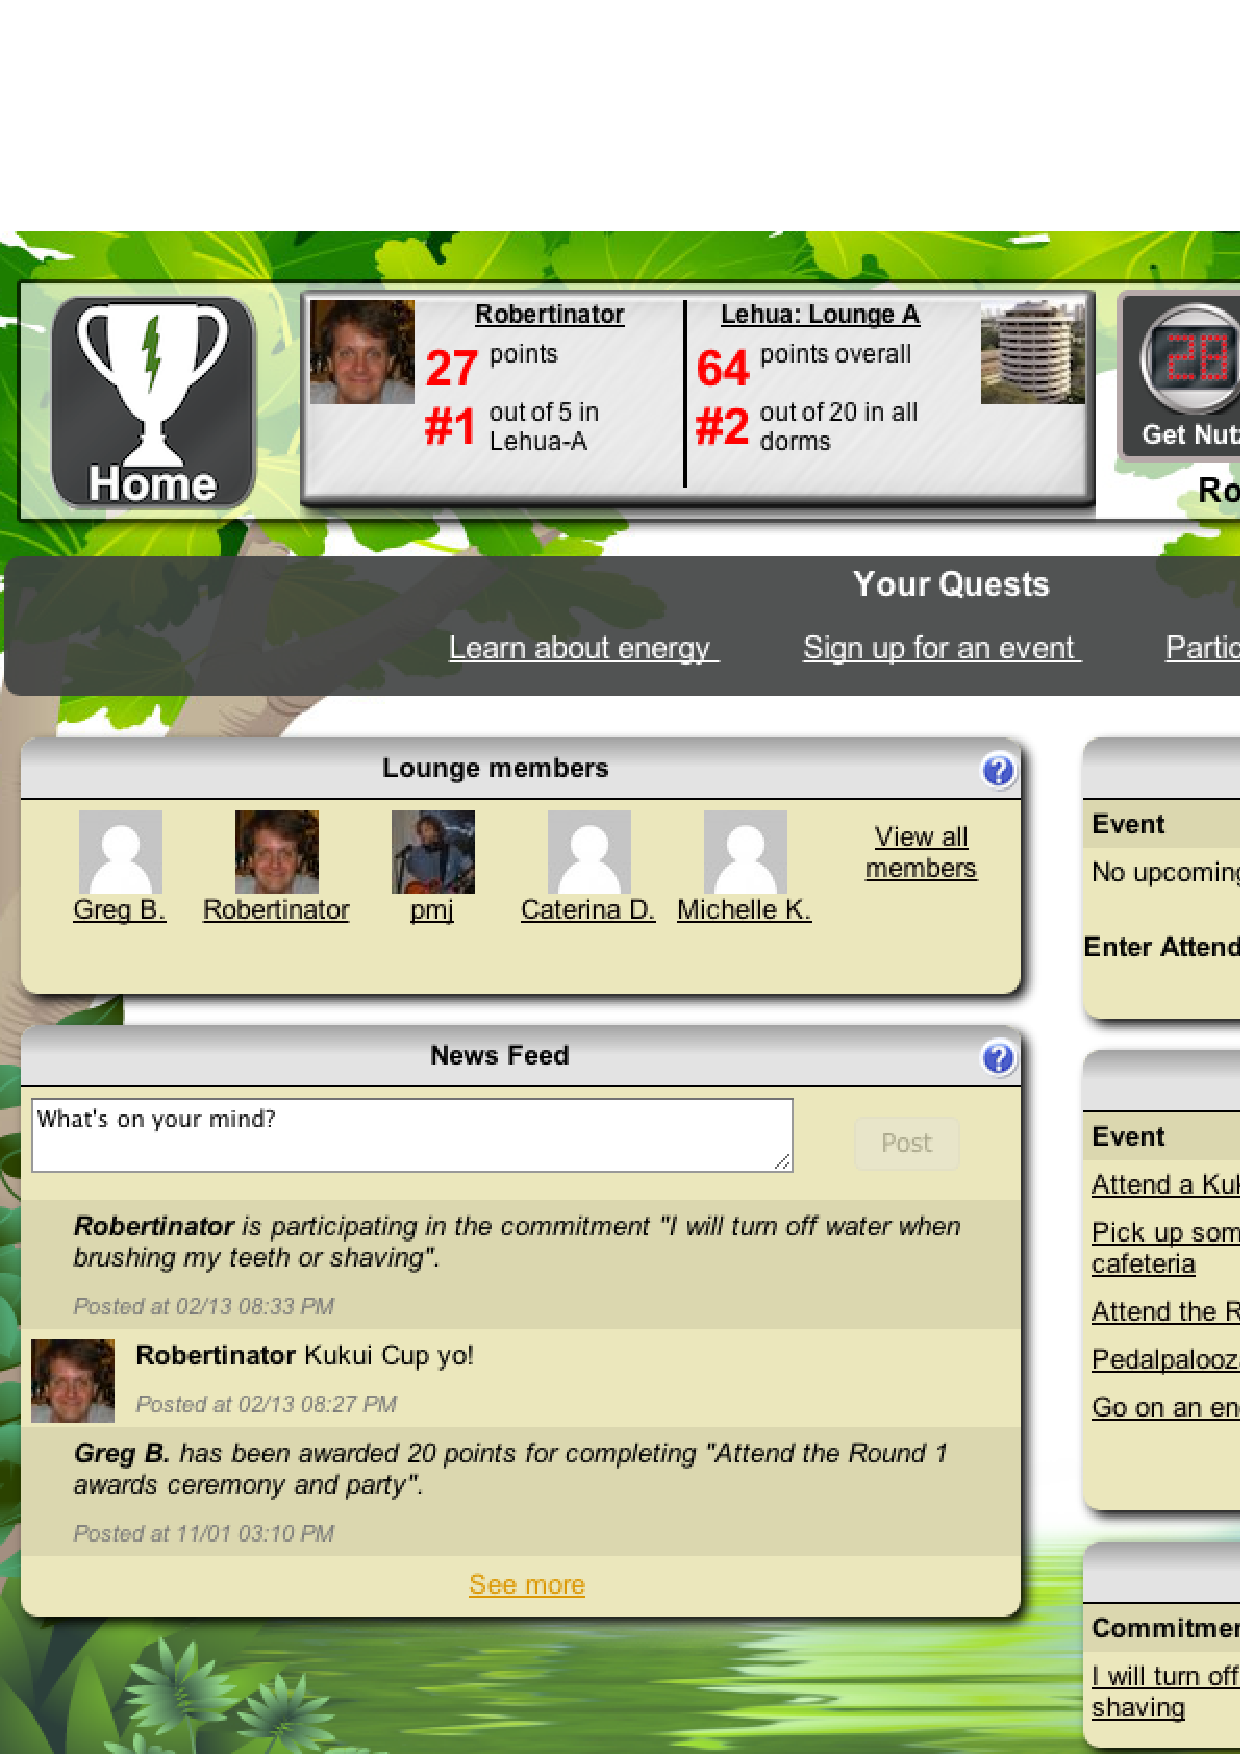
\includegraphics[width=\textwidth]{news-page}
		\caption{The News page of the challenge website}
\label{fig:news-page}
\end{figure}

The left column shows two widgets: Lounge members and News Feed. The Lounge members widget shows a subset of the participants in the lounge along with their selected profile picture, with a link to a page showing all the members. The News Feed provides a simple discussion board for lounge members similar to the `wall' concept on Facebook. Participants could type in messages that would be displayed to all other members of the lounge, in reverse chronological order. The system created automated posts when participants performed an action like making a commitment or earning points.

The right column shows three widgets: Upcoming Events, Most Popular, and My Public Commitments. The Upcoming Events widget shows any events taking place today or in the next 7 days. After an event, participants can enter their attendance code directly into the text field to receive points without having to navigate to the specific event page.

The Most Popular widget cycles through a list of events, activities, and commitments ranked in order of how many participants have performed those actions. This widget is intended highlight the popular actions and encourage participants to take part in them. The My Public Commitments widget simply lists the commitments that the participant, which is intended as a reminder to live up to the commitments.


\subsubsection{Prizes Page}

The Prizes page showed participants more information about the incentives available in the challenge. \autoref{fig:prizes-page} shows a portion of the Prizes page from the Overall Round of the challenge.

\begin{figure}[htbp]
	\centering
		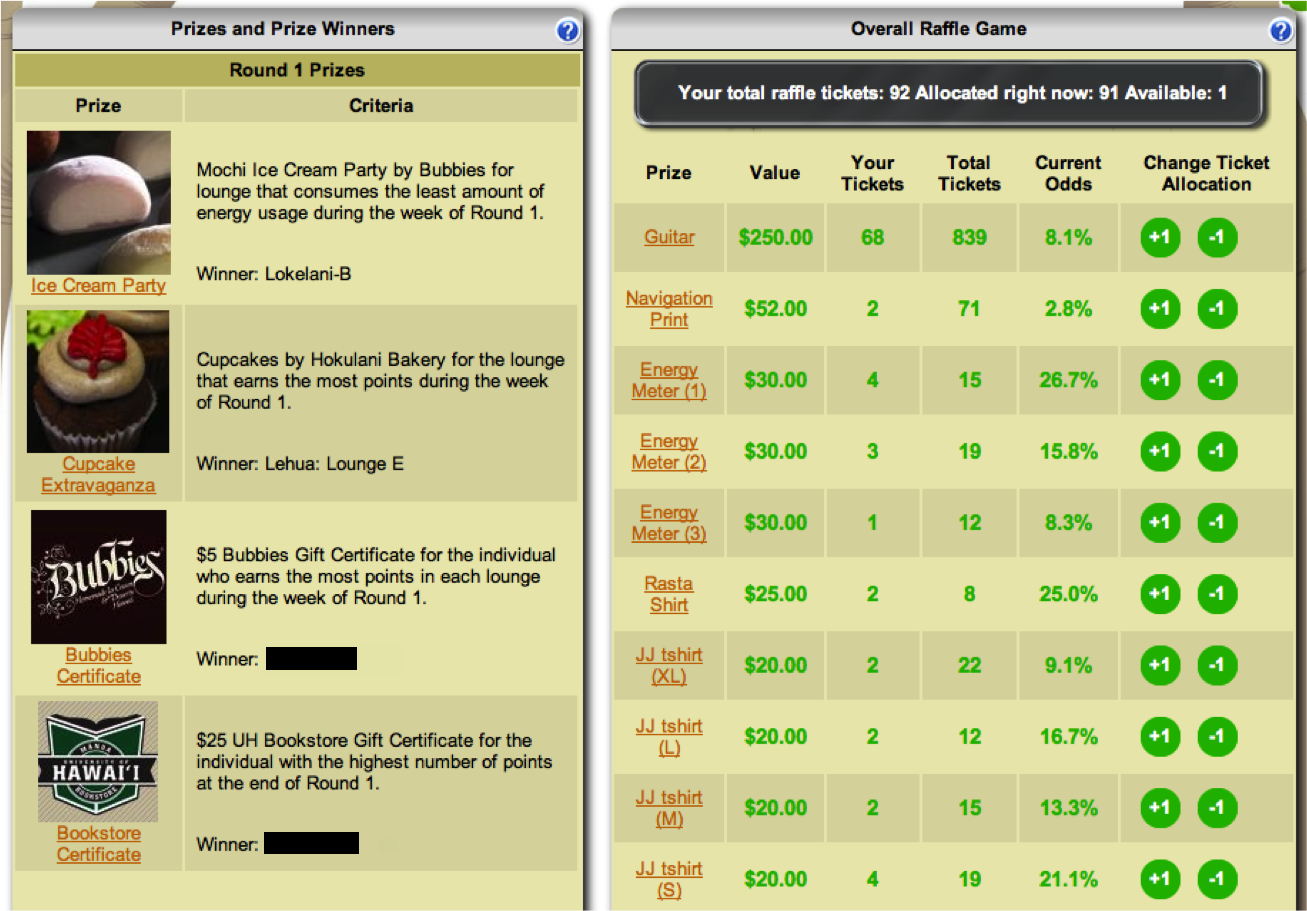
\includegraphics[width=\textwidth]{prizes-page}
		\caption{An excerpt from the Prizes page of the challenge website}
\label{fig:prizes-page}
\end{figure}

The left side of the Prizes page shows the prizes awarded to the top participants in each category, as described in \autoref{sec:prizes}. For each prize, the widget showed the lounge or individual in first place for that competition (the currently projected winner). The right side of the prizes page showed the Raffle Game described in \autoref{sec:raffle-game}.


\subsubsection{Profile Page}

The Profile page allowed participants to edit their personal information and view data about their progress in the game. \autoref{fig:profile-page} shows what the Profile page looks like.

\begin{figure}[htbp]
	\centering
		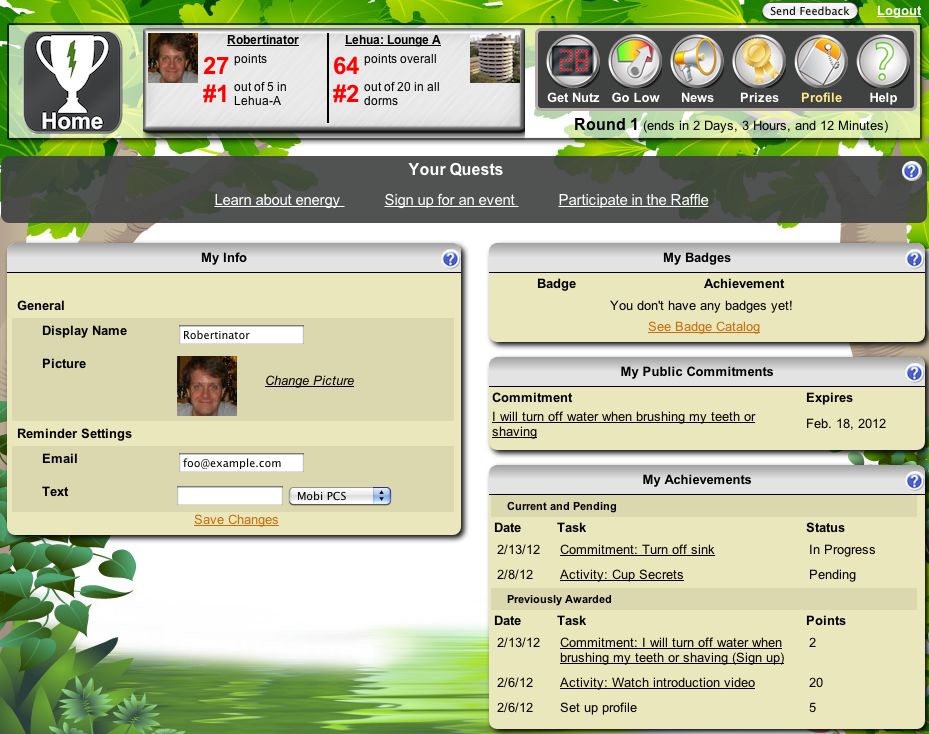
\includegraphics[width=\textwidth]{profile-page}
		\caption{The Profile page of the challenge website}
\label{fig:profile-page}
\end{figure}

The left side of the page contains the My Info widget. In My Info, participants could change their display name (used to identify the participant on the website, such as on scoreboards or the lounge News Feed), profile picture, and contact information used when event reminders were requested.

The right side of the page shows challenge information for the participant: My Badges, My Public Commitments, and My Achievements. Participants could earn badges for reaching certain goals, such as making five commitments, and the badges earned were displayed in the My Badges widget. My Public Commitments shows the participants commitments (also shown on the News page). My Achievements showed a complete record of all actions taken by the participant in the challenge and all points earned.


\subsubsection{Help Page}

The Help page is shown in \autoref{fig:help-page}. On the left side of the page showed the introductory video and links to the rules of the challenge. On the right side, one widget showed links to frequently asked questions, and the Ask an Admin widget. Ask an Admin allowed participants to send questions to the challenge administrators, which was delivered by email. The Ask an Admin functionality was also available on every page of the website using the Send Feedback button at the top right corner of the page.

\begin{figure}[htbp]
	\centering
		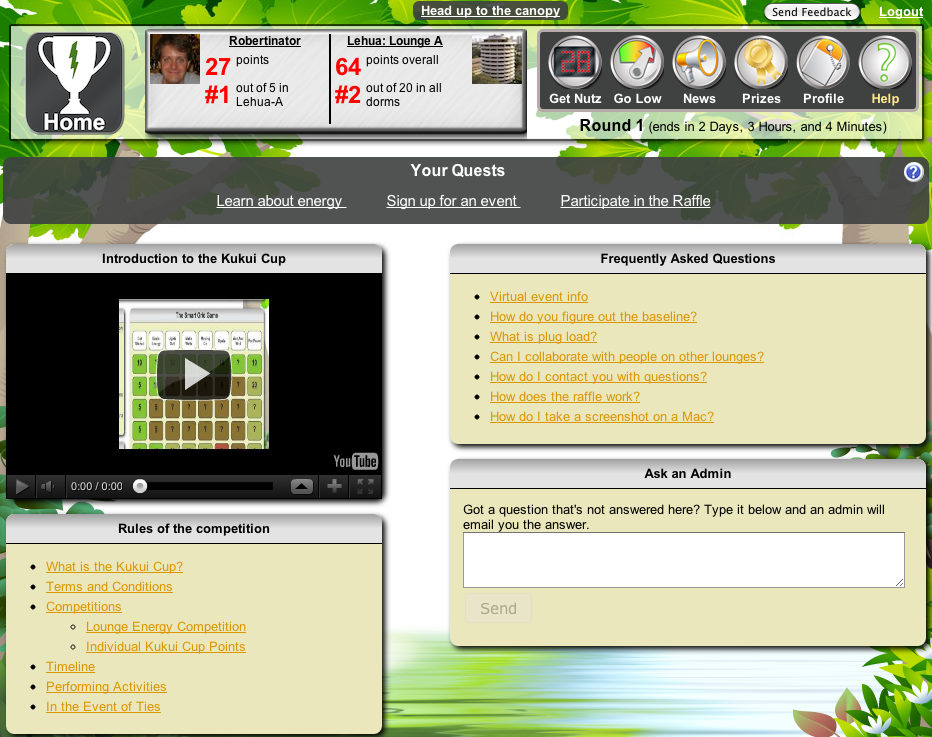
\includegraphics[width=\textwidth]{help-page}
		\caption{The Help page of the challenge website}
\label{fig:help-page}
\end{figure}


\subsubsection{The Canopy}

The Canopy was an area of the website designed to provide an additional level of experience for the top participants in the challenge. The background of the challenge website featured a forest theme, so the Canopy was named to convey that it existed above the rest of the website. Many games feature different levels of difficulty\fxnote{reference for levels of difficulty in games?}, something that was not addressed in the Smart Grid Game. The Canopy was conceived as a way to keep the top participants engaged even if they had earned most of the points available in the Smart Grid Game.

The Canopy was intended to be introduced to top players at the beginning of Round 2 of the challenge. The top 50 participants would be sent an email inviting them to a new part of the website. In keeping with the Canopy motif, Canopy members would access the Canopy page by finding a hidden link at top of each web page. The link was hidden until the Canopy member's mouse moved over the link, at which point it was displayed permanently. The ``Head up to the Canopy'' link can be seen at the top of \autoref{fig:help-page}.

\begin{figure}[htbp]
	\centering
		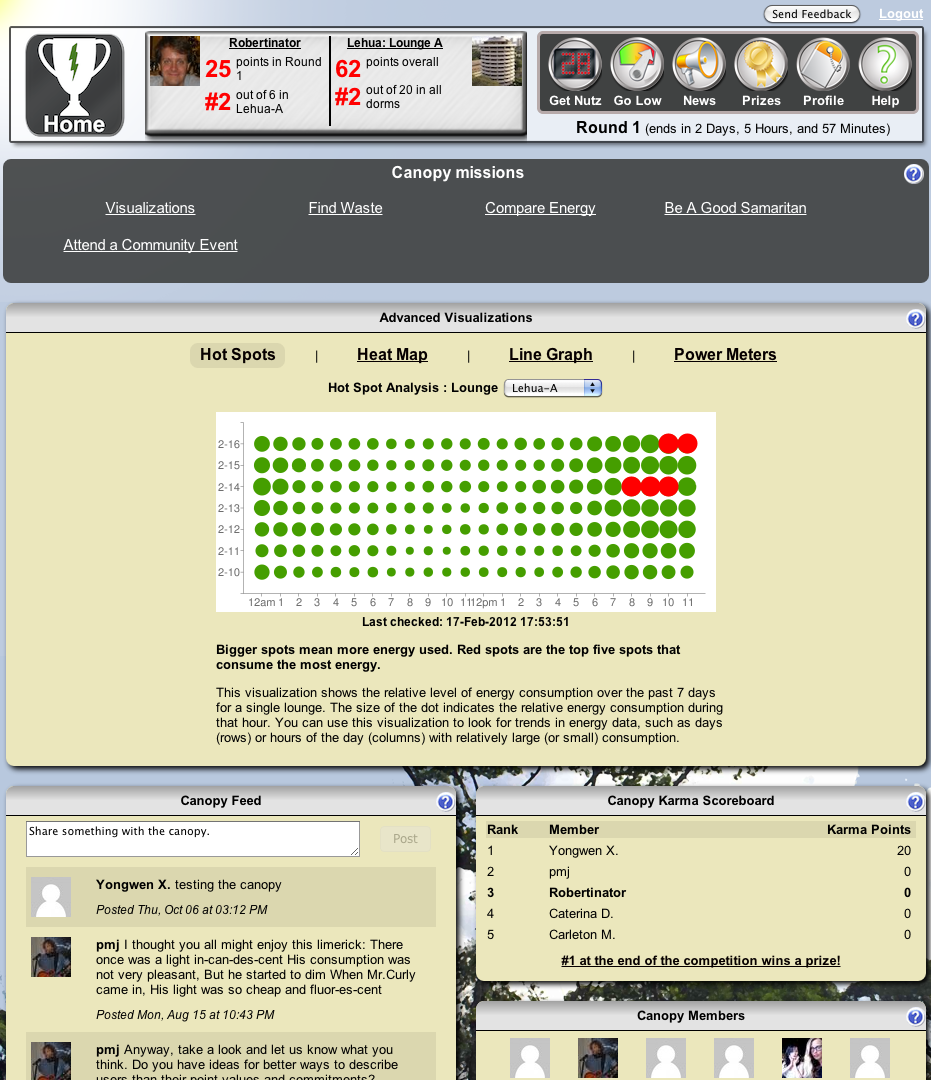
\includegraphics[width=\textwidth]{canopy-page}
		\caption{The Canopy page of the challenge website}
\label{fig:canopy-page}
\end{figure}

\autoref{fig:canopy-page} shows the Canopy page itself. The Canopy provided a series of missions, which were displayed just under the header in a similar fashion to the quests in the forest portion of the website. Some Canopy missions were to be accomplished individually, while other missions required two or three participants to work together. Participants could indicate that they were ``up'' for a group mission to find other interested participants.

The Canopy missions contained links to Canopy activities. Canopy activities were like forest activities (see \autoref{sec:activities}), but instead of earning points upon completion, Canopy activities earn \emph{Canopy Karma}, which was a separate point system for the Canopy. Canopy Karma was used instead of the standard points to ensure that the Canopy itself did not unbalance the point competition by providing a way for the top players to earn more points that were not available to the rest of the participants.

The energy data and visualizations shown on the Go Low page were deliberately simple to avoid confusing participants, based on the results of usability testing. In addition, the detailed energy data shown on Go Low comes only from the participant's lounge. Since the Canopy was intended for the top participants of the challenge, who were believed to be more receptive to detailed energy data and data for other lounges, energy visualizations feature prominently in the Canopy. Several of the Canopy activities involved looking at the advanced visualizations and answering questions based on their understanding of the data.

Since the members of Canopy cut across different lounges, a special Canopy Feed discussion board was provided to allow collaboration. The Canopy Feed worked in the same way the lounge News Feed described in \autoref{sec:news-page}. The Canopy also featured a Canopy Karma scoreboard showing the top participants in the Canopy, and a \$25 UH Bookstore gift card was offered as a prize to the participant with the most Canopy Karma at the end of the challenge.


\subsection{Energy Data Integration}
\label{sec:energy-data-integration}

The energy data for the challenge was stored in a WattDepot server. Before and during the challenge, the energy meters were queried at approximately 15 second intervals. After the challenge was over, there was no need for real-time data, so I changed the query interval to 5 minutes.

The challenge website has several areas that require access to energy and power data: the Daily Energy Goal Game, the Current Power gauge, and the Energy Scoreboards. Since each of these components run in the browser and dynamically update, the load on the WattDepot server could be proportional to the number of participants in the challenge. To reduce the potential load on on the WattDepot server, Professor Philip Johnson wrote a system called WattDepot-GData~\cite{wattdepot-gdata}, which periodically queries a WattDepot server and stores the results in a Google Docs spreadsheet. The spreadsheets created by WattDepot-GData are structured to meet the needs of the Makahiki visualizations, such as the total energy use since the beginning of the current round of the challenge. Using Google Docs to store the data in the cloud also insulates the WattDepot server from heavy client loads.
